\documentclass[a4paper, 10pt]{article}

\usepackage{tabularx} % extra features for tabular environment
\usepackage{amsmath}  % improve math presentation
\usepackage{graphicx} % takes care of graphic including machinery
\usepackage[margin=1in,letterpaper]{geometry} % decreases margins
\usepackage{cite} % takes care of citations
\usepackage[final]{hyperref} % adds hyper links inside the generated pdf file
\usepackage{ctex}
\usepackage{titlesec}
%\usepackage{CJKutf8, CJK}
\usepackage{makecell}                 % 三线表-竖线
\usepackage{booktabs}                 % 三线表-短细横线
% \usepackage{natbib}
\usepackage{graphicx}				  % 表格单元格逆时针
\usepackage{multirow}				  % 合并单元格
\usepackage{array}
\usepackage{amssymb}				  % 勾
\usepackage{amsmath}
\usepackage{longtable}                % 导入 longtable 宏包,表格自动换行
\usepackage{caption}
\usepackage{subcaption}               % 设置子图
\usepackage{color}					  % 文本颜色包
\usepackage{xcolor}
\usepackage{bbm}					  % 输入指示函数
\usepackage{tablefootnote}			  % 表格注释
\usepackage{pythonhighlight}
\usepackage{fancyhdr}
\usepackage{lastpage}
\pagestyle{fancy}
\fancyhf{}
\fancyhead{}
\fancyfoot{}
\fancyhead[R]{\small Page \thepage\ of \pageref*{LastPage}}
\fancyhead[L]{\small Report}

\usepackage{listings}                 % 导入代码块
\usepackage{xcolor}
\lstset{
	numbers=left, 
	tabsize=1,
	columns=flexible, 
	numberstyle=  \small, 
	keywordstyle= \color{ blue!70},
	commentstyle= \color{red!50!green!50!blue!50}, 
	frame=shadowbox, % 阴影效果
	rulesepcolor= \color{ red!20!green!20!blue!20} ,
	escapeinside=``, % 英文分号中可写入中文
	xleftmargin=2em,
	xrightmargin=2em, 
	aboveskip=1em,
} 

\hypersetup{
	colorlinks=true,       % false: boxed links; true: colored links
	linkcolor=blue,        % color of internal links
	citecolor=blue,        % color of links to bibliography
	filecolor=magenta,     % color of file links
	urlcolor=blue         
}
%++++++++++++++++++++++++++++++++++++++++
\titleformat{\section}{\Large\bfseries\songti}{\thesection}{1em}{}
\titleformat{\subsection}{\large\bfseries\songti}{\thesubsection}{1em}{}
\titleformat{\subsubsection}{\normalsize\bfseries\songti}{\thesubsubsection}{1em}{}
\titleformat{\paragraph}{\small\bfseries\songti}{\paragraph}{1em}{}
\titleformat{\subparagraph}{\footnotesize\bfseries\songti}{\subparagraph}{1em}{}

\begin{document}
	
	
	\title{\songti \zihao{4}9月13日-9月20日工作汇报}
	\author{\textrm{Ku Jui}}
	\date{\textrm{September 2023}}
	\maketitle
	
	\renewcommand{\figurename}{Figure} % 可以重新定义abstract,因为ctex会覆盖thebibliography
	% 	\begin{abstract}
		%		In this experiment we studied a very important physical effect by measuring the
		%		dependence of a quantity $V$ of the quantity $X$ for two different sample
		%		temperatures.  Our experimental measurements confirmed the quadratic dependence
		%		$V = kX^2$ predicted by Someone's first law. The value of the mystery parameter
		%		$k = 15.4\pm 0.5$~s was extracted from the fit. This value is
		%		not consistent with the theoretically predicted $k_{theory}=17.34$~s. We attribute %this
		%		discrepancy to low efficiency of our $V$-detector.
		%	\end{abstract}
	\renewcommand{\contentsname}{Contents}
	\renewcommand{\tablename}{Table}
	\tableofcontents  % 自动生成目录
	
	\part{Pre-Knowledge}	
	
	\section{方向}
	
		边缘检测\footnote{人类视觉系统对边缘高度敏感,保留结构信息对图像重建任务的性能至关重要。定义边缘可以通过学习区分黑暗区域的不同物体来指导增强过程,而不仅仅是识别低光区域。通过保留图像中的颜色和结构属性,这使得物体之间的可见性更好。}:
		
		\begin{itemize}
			\item[(1)] 
			手工设计各种滤波器来生成边缘图。
			
			\item[(2)]
			根据人类设计的特征使用数据驱动模型来预测边缘(随机决策森林来学习边缘斑块)
			
			\item[(3)]
			深度学习方法从原始数据中学习复杂的特征表示端到端边缘检测模型。
		\end{itemize}	
		
		\cite{rana2021edge}与\cite{zhu2020eemefn}在暗区域中加入敏感边缘先验可以降低优化外观重构时的不适定程度。

		这个边缘检测的思想目前的文献调研显示只集中在边缘检测和外观指导图像恢复,没有考虑和图像的色彩结合,以及恢复出来的图像还是有明显噪点。
		
		\subsection{问题} 
		
		目前的文献研究表明,在弱光环境下的图像恢复中,采用边缘检测思想来引导弱光图像恢复过程的方法,一般的策略是将边缘图与初步恢复的图像进行串联,然后通过单一的增强网络来实现最终的图像恢复。恢复结果的质量往往受到最后的增强网络设计和初步恢复图像所包含特征与真实图像特征之间的相似度的影响。
		
		初步恢复的方法目前主要包括两种:一种是利用多曝光技术获得具有不同曝光度的图像,然后结合恢复网络进行初步恢复;另一种则是直接通过神经网络进行弱恢复,但由于噪声和伪影的存在,以及色彩与真实图像之间的差异,结果通常并不理想。
		
		在增强网络的设计方面,主要采用了两种主要架构:StyleGAN 和 U-Net。这些网络通常通过串联操作或将边缘图像的分块作为卷积核的方式来引导图像恢复过程。
		
		此外,获得边缘图的方法也各不相同,一般采用边缘检测网络来生成边缘图。Canny 和 Sobel 算子通常被用作对比实验,也有一些研究采用辅助边缘网络以提高边缘图生成的准确性。这些方法在弱光图像恢复研究中都具有一定的学术和实际应用价值。
		
		\subsection{创新想法}
		
		在目前的研究中,我们探索了不同的边缘图生成方法,并引入了基于 VGG 网络的方法,同时采用 Canny 边缘检测作为参考对比方法。我们的主要目标是设计一种综合恢复策略,结合了以下几个关键元素:边缘图、初步恢复图以及原始图像的 Y/Cb/Cr 通道信息。
		
		在初步恢复图的生成方面,我们采用了一种复合型卷积神经网络 CNN 与 Transformer 网络的混合模型,见 Fig.\ref{fig: First Architecture}。这一模型旨在从弱光图像中提取长距离和短距离特征,以更全面地捕捉图像的信息。通过特定的特征融合策略,我们期望能够得到初步恢复的图像。
		
		至于增强网络的设计,我们目前尚未确定具体的方法。然而,我们的研究侧重于构建一个整体恢复框架,该框架利用边缘图、初步恢复图和通道信息的融合,以提高弱光图像的质量。我们将继续探索合适的增强网络结构,以进一步提升恢复结果的性能。这一研究旨在为弱光图像恢复领域提供新的理论和方法,以改善图像质量并拓展应用领域。
		
		\begin{figure}[htbp]
			% read manual to see what [ht] means and for other possible options
			\centering 
			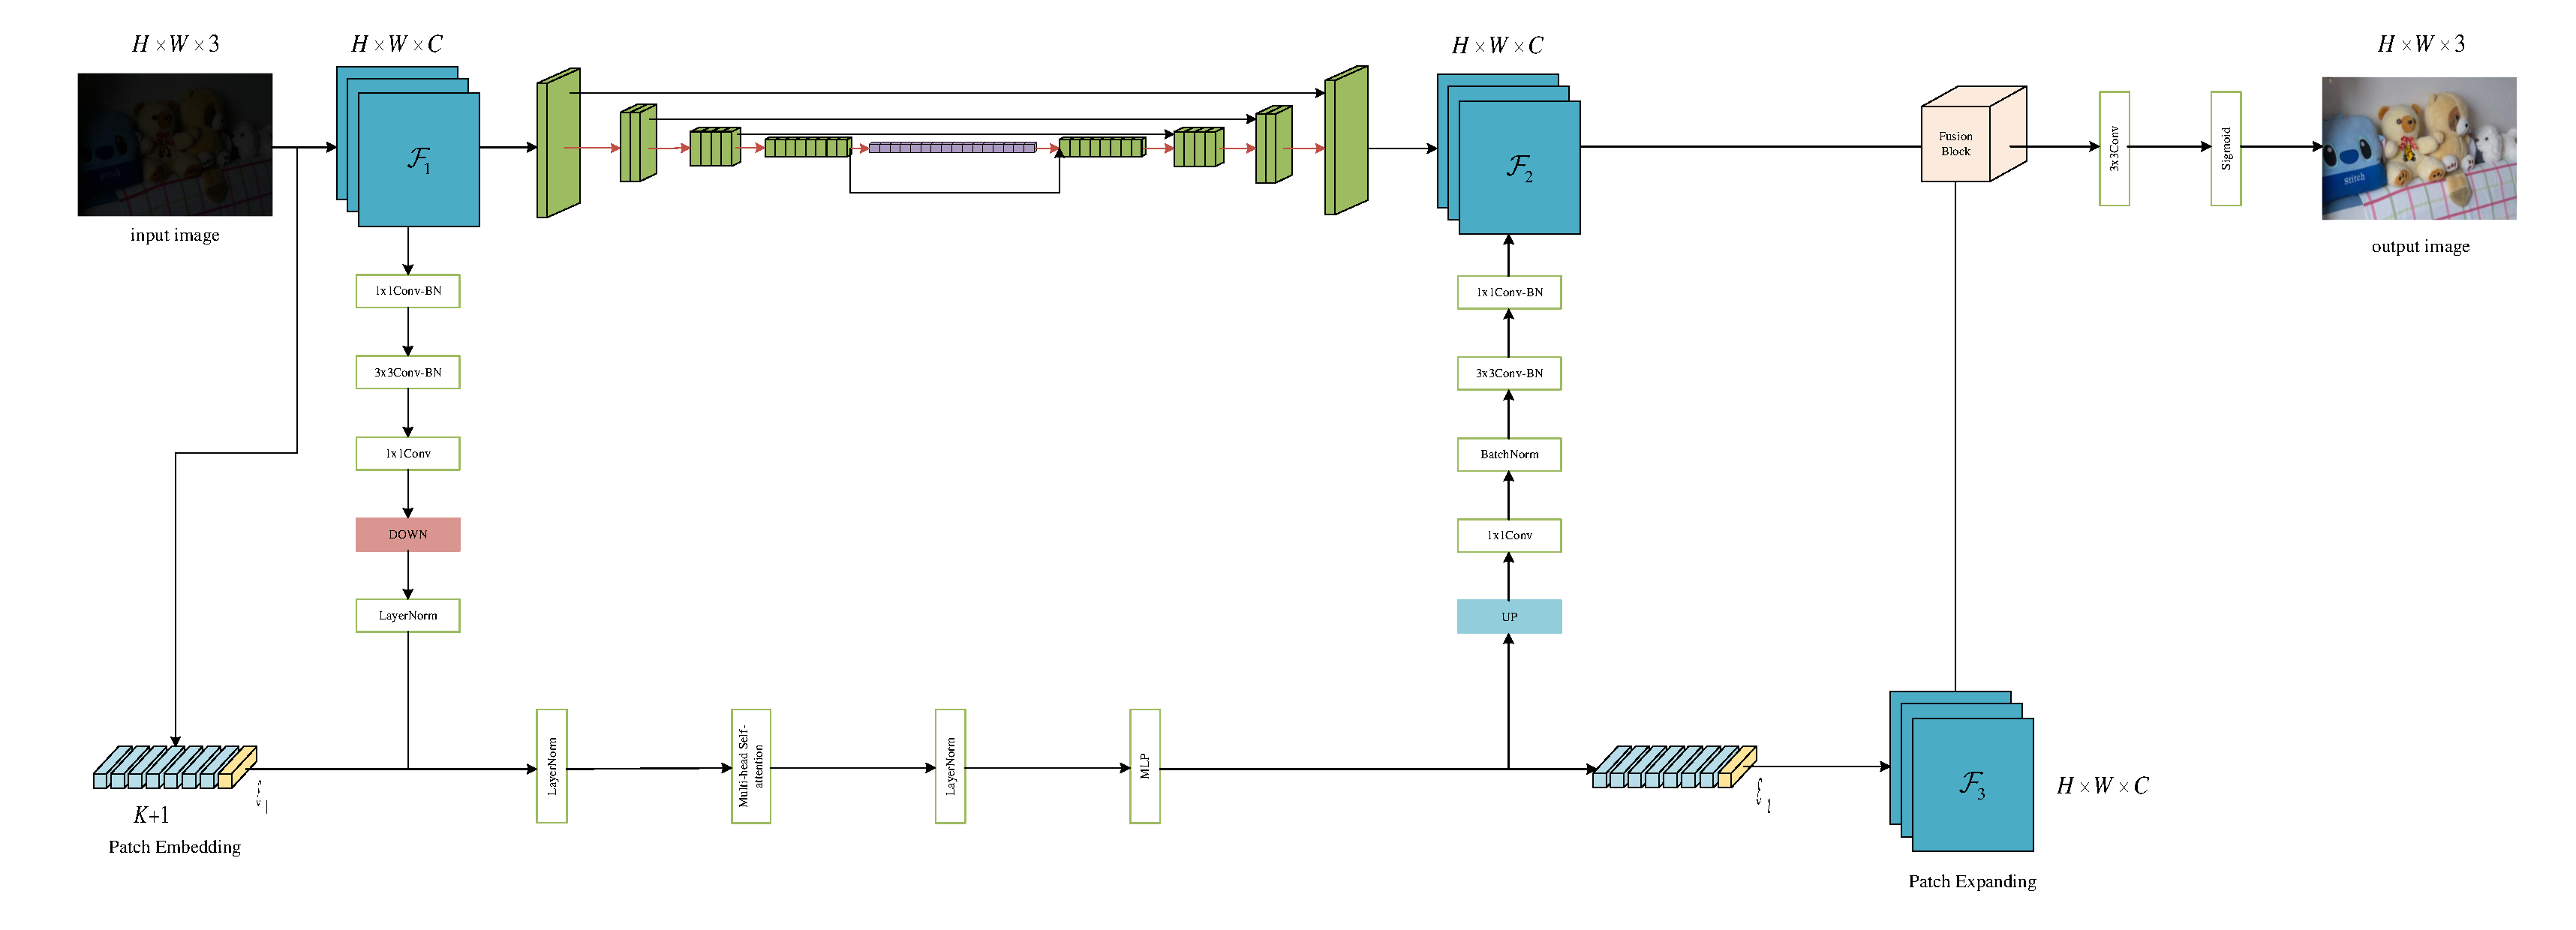
\includegraphics[width=\columnwidth]{picture/LLIE/First architecture}
			%\captionsetup{font=scriptsize}
			\caption{
				\label{fig: First Architecture} 
				Low-Lighting 图像恢复网络,其采用一个 U-Net 和 ViT 的并行架构,通过 U-Net 结构得到一个弱恢复的弱特征图 $\mathcal{F}_2$,通过 ViT 融合的特征可以初步增强弱特征图 $\mathcal{F}_2$,ViT 的输出经过 Patch Expanding 的特征图 $\mathcal{F}_3$ 经过与 U-Net 输出的特征图 $\mathcal{F}_2$ 融合之后得到一个初步恢复的图片 output image,用以后续参与图片的进一步恢复
			}
		\end{figure}
		
		\paragraph{Attention in CV}
		
		在计算机视觉领域,研究人员使用了不同类型的注意力机制,目的是使模型聚焦于图像本身。这大致分为两种类型:一种是基于通道的注意力机制,即 Squeeze-and-Excite。另一个是基于空间的注意力机制\cite{woo2018cbam}。然而,研究发现这些类型有三个局限性:
		
		\begin{itemize}
			\item[(1)] 
			卷积捕捉远距离特征的能力较差;
			
			\item[(2)]
			注意力机制关注所有输入;当分辨率较大时,计算成本增加;
			
			\item[(3)]
			不同时关注通道和空间维度关注信息。这就造成了信息的浪费和注意力的减弱。
		\end{itemize}	
		
		针对第一个限制 \cite{ramachandran2019stand} 将所有卷积替换为独立的自注意层和空间意识的独立自注意层,替换后的模型为纯注意模型。纯注意模型增强了网络对远距离特征连接的建模能力。在 ImageNet分类任务和 COCO 对象检测任务中,该模型优于使用卷积的基线模型。对于第三个限制,Woo 等人\cite{woo2018cbam}提出了一种卷积块注意模型 CBAM,这是一种轻量级的通用注意模型。该模型从通道维度和空间维度两方面关注重要信息。由于 CBAM 从多个维度提取重要信息,该模型被广泛应用于目标检测、目标分类等任务。实验表明,CBAM 模块可以显著提高网络的表达能力。
		
		\paragraph{U-Net for LLIE}
		
		U-Net 网络由卷积层、下采样、上采样和跳过连接操作组成,其编码器和解码器具有对称结构。长期以来,U-Net 网络及其改进结构由于其强大的特征学习和特征重构能力,在图像语义分割领域取得了巨大的成功。U-Net 网络在弱光图像增强方面显示出出色的效果。Chen 等\cite{chen2018learning}创新性地提出了一种基于 U-Net 框架的弱光图像增强网络。该网络的核心架构是多尺度上下文聚合网络 (CAN) 和 U-Net 网络。之后的工作\cite{chen2018learning, zamir2021learning}也将 U-Net 架构应用到自己的网络中,其网络包含两个子网。即图像约简子网和感知损失子网,其中图像约简子网具有与\cite{chen2018learning}相同的 U-Net 架构。虽然\cite{chen2018learning, zamir2021learning}在使用U-Net架构增强图像方面取得了一定的效果,但\cite{meng2020gia}认为\cite{chen2018learning, zamir2021learning}网络忽略了全局信息,导致增强图像中的颜色不自然和物体伪影问题。为了改善以往网络的缺陷,利用 U-Net 架构,\cite{meng2020gia}在U-Net的编码器和解码器之间增加了全局信息感知模块(global information awareness module, GIA), GIA 可以将全局信息整合到整个网络中,改善增强图像中的颜色不一致和伪影。经过对\cite{chen2018learning, meng2020gia, zamir2021learning}的仔细研究,基于 U-Net 网络的弱光图像增强方法取得了很好的效果。然而,该网络仍然存在两个局限性:
		
		\begin{itemize}
			\item[(a)] 
			跳过连接只融合相同尺度的特征,导致编码器和解码器之间存在较大的语义差距;
			
			\item[(2)]
			全局上下文信息的连接相对稀缺。
		\end{itemize}	
		
		这两个限制容易导致增强图像的细节丢失、对比度差和颜色信息不准确。Zhou等\cite{zhou2018unet++,zhou2019unet++}改进了 U-Net 架构生成 U-Net++,在 U-Net++ 中将跳跃连接重新设计为一系列嵌套的密集跳跃连接,实现了多个特征的融合,加强了不同层次的特征信息接触。

		\paragraph{CNN for LLIE}
		
		CNN 在许多计算机视觉任务中表现出了令人印象深刻的结果。CNN 利用注意力机制\cite{yang2021locally, zhang2020attention}和上下文信息,从原始图像中生成注意感知并提取多尺度特征\cite{li2018multi,zamir2020learning}。基于 CNN 的低光图像增强方法不断发展。例如,基于 CNN 的自适应弱光图像增强框架\cite{li2020visual}极大地增强了图像对比度、颜色和细节信息。然而,现有的基于 CNN 的方法大多侧重于图像亮度、纹理和颜色的恢复\cite{xu2020learning}。由于局部光照不均匀,颜色信息和细节信息丢失严重,容易出现过增强或增强不足的问题。
		
%%%%%%%%%%%%%%%%%%%%%%%%%%%%%%%%%%%%%%%%%%%%%%%%%%%%%%%%%%%%%%%%%%%%%%%%%%%%%%%%%%%%%%%%%%%%%%%%%%%%
%%%%%%%%%%%%%%%%%%%%%%%%%%%%%%%%%%%%%%%%%%%%%%%%%%%%%%%%%%%%%%%%%%%%%%%%%%%%%%%%%%%%%%%%%%%%%%%%%%%%
%%                                                                                                %% 
%%								          Paper reading                                           %%
%%                                                                                                %%
%%%%%%%%%%%%%%%%%%%%%%%%%%%%%%%%%%%%%%%%%%%%%%%%%%%%%%%%%%%%%%%%%%%%%%%%%%%%%%%%%%%%%%%%%%%%%%%%%%%%
%%%%%%%%%%%%%%%%%%%%%%%%%%%%%%%%%%%%%%%%%%%%%%%%%%%%%%%%%%%%%%%%%%%%%%%%%%%%%%%%%%%%%%%%%%%%%%%%%%%%	

	
	\part{Paper Reading}
	
	\section{LLIE}
		
		\subsection{(2023.1)LAE-Net: A locally-adaptive embedding network for low-light image enhancement}
		
		\paragraph{LAE-Net:一种用于弱光图像增强的局部自适应嵌入网络}
		
		\paragraph{(Pattern Recognition 2023 1区) doi: 10.1016/j.patcog.2022.109039}
		
			\subsubsection{Research Background}
			
			由于相机成像机制的本质特性,在弱光或背光环境下拍摄的图像通常会出现对比度低、细节不可见、噪声强烈等视觉质量下降的问题。
			
			在弱光增强任务中,如何平衡光强、细节呈现和色彩保真度的图像增强特性是一个主要的挑战。在自然场景中,频率和光照特征\footnote{频率特征反映了图像中灰度变化的剧烈程度,是灰度在平面空间上的梯度。例如,大面积的沙漠在图像中是一片灰度变化缓慢的区域,对应的频率值很低;而对于地表属性变换剧烈的边缘区域在图像中是一片灰度变化剧烈的区域,对应的频率值较高;光照特征则反映了图像中光线照射的情况。在自然环境中,光照条件可能会随着时间、天气等因素发生变化,从而影响到图像的光照特征。由于这些因素的影响,频率和光照特征在空间域中的分布可能会呈现出复杂和多样的模式。}在空间域中的多重分布使得平衡更加困难。
			
			\subsubsection{Contribution}
			
			文章提出,从人的视觉系统来看,噪声在图像的平滑区域(低频为主,即熵值大的区域)更加显眼而在高频区域则由于人的视觉掩盖机制(人眼无法同时接受太多信息从而有选择性地忽略一些信息)而相对不显眼。
			
			作者提出了一种局部自适应嵌入网络,即 LAE-Net, 通过局部自适应核选择和多分布问题的特征自适应来实现高质量的低光图像增强。
			
			\begin{itemize}
				\item[(1)] 
				针对频率多分布,作者重新思考人眼的空间-频率特征,实验探索了感受野大小、图像空间频率和光增强特性之间的关系,并提出了一种熵启发的核选择卷积,其中每个神经元可以根据其信息熵特征的空间频率自适应调整感受野大小。
				
				\item[(2)]
				对于光照多分布,作者提出了一个光照关注转移子网,神经元可以同时感知全局一致性和局部细节,并相应地提示需要关注的地方,从而调整改进后的特征。
				
			\end{itemize}	
			
			\subsubsection{Approach}
			
			作者提出了两个模块,一个 EIKS 模块用局部熵来代表图像的局部频率特性,利用熵图来指导卷积的感受野\footnote{感受野 (Receptive Field) 在卷积神经网络中,是指特征图上某个元素的计算受输入图像上某个区域的影响,这个区域即该元素的感受野}(文章认为高频噪声不突出,用小感受野,低频噪声突出,用大感受野);另一个是基于 illumination map 来做注意力的 IAT 模块
			
			\subsubsection{Future}
		
			-
			
		\subsection{(2023.1)LACN: A lightweight attention-guided ConvNeXt network for low-light image enhancement}
			
		\paragraph{LACN:采用一种轻量级的注意力引导的对流网络来增强弱光图像}
			
		\paragraph{(Engineering Applications of Artificial Intelligence 2区) doi: 10.1016/j.engappai.2022.105632}
			
			\subsubsection{Research Background}
				
			在弱光图像增强任务中,通常在增强图像亮度的同时放大了暗区的噪声。目前,许多深度学习方法在这一阶段并不能有效地抑制噪声并捕获重要的特征信息。
			
			\subsubsection{Contribution}
			
			本文提出了一种新的轻量级注意力引导卷积神经网络 (LACN),该网络 (如 Fig. \ref{fig: LACN model structure} 所示) 不仅可以提高图像对比度和抑制噪声,还可以增强图像的颜色信息保留能力和细节恢复能力。
			
			\begin{figure}[htbp]
				% read manual to see what [ht] means and for other possible options
				\centering 
				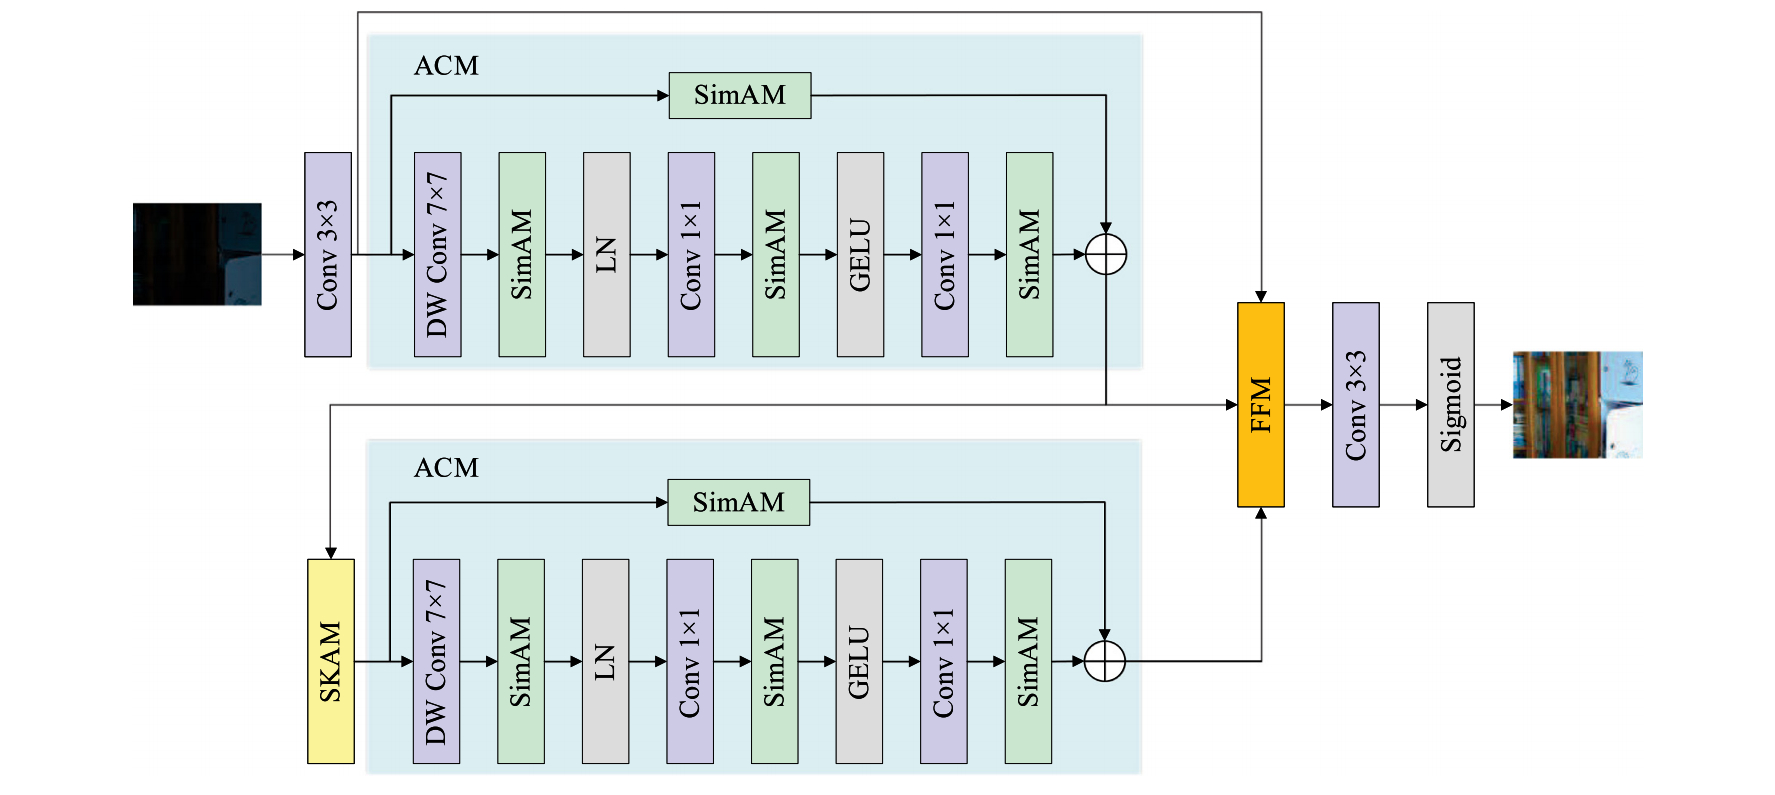
\includegraphics[width=\columnwidth]{picture/LLIE/LACN/LACN model structure}
				%\captionsetup{font=scriptsize}
				\caption{
					\label{fig: LACN model structure} 
					Model structure of LACN. The brief process is to first perform shallow feature extraction on the image, then send it to ACM to extract features, enter ACM again after passing SKAM, moreover send the features extracted twice by ACM and shallow features into FFM, and finally carry out feature reconstruction to get an enhanced image.
				}
			\end{figure}
			
			主要贡献如下:
			
			\begin{itemize}
				\item[(1)] 
				通过在 ConvNeXt 骨干网中引入注意力机制,提出了一种新的 ACM。针对该模块,通过对两个 ACM 的叠加和特征融合,建立了一种基于多注意机制的新型轻量级网络 LACN;
				
				\item[(2)]
				设计的 SKAM 是非平凡的,可以有效地提取全局和局部信息。因此,在实现感受野自适应调节的同时,有利于对整个图像的光照条件进行评价;
				
				\item[(3)]
				采用两个跳线连接,使浅层特征可以反向传播。利用特征融合模块 (Feature Fusion Module, FFM) 融合不同层的特征 (如 Fig .\ref{fig: FFM structure} 所示),保留丰富的颜色信息,减少颜色信息的丢失;
			\end{itemize}	
			
			\begin{figure}[htbp]
				% read manual to see what [ht] means and for other possible options
				\centering 
				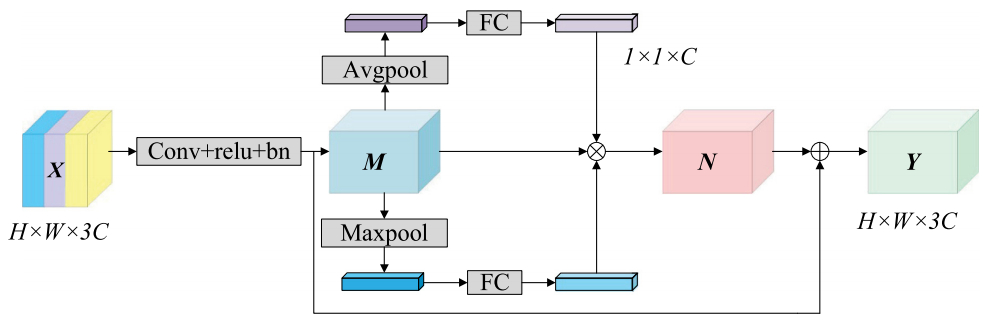
\includegraphics[width=0.8\columnwidth]{picture/LLIE/LACN/FFM structure}
				%\captionsetup{font=scriptsize}
				\caption{
					\label{fig: FFM structure} 
					Structure of feature fusion module.
				}
			\end{figure}
			
%			\begin{figure}[htbp]
%				% read manual to see what [ht] means and for other possible options
%				\centering 
%				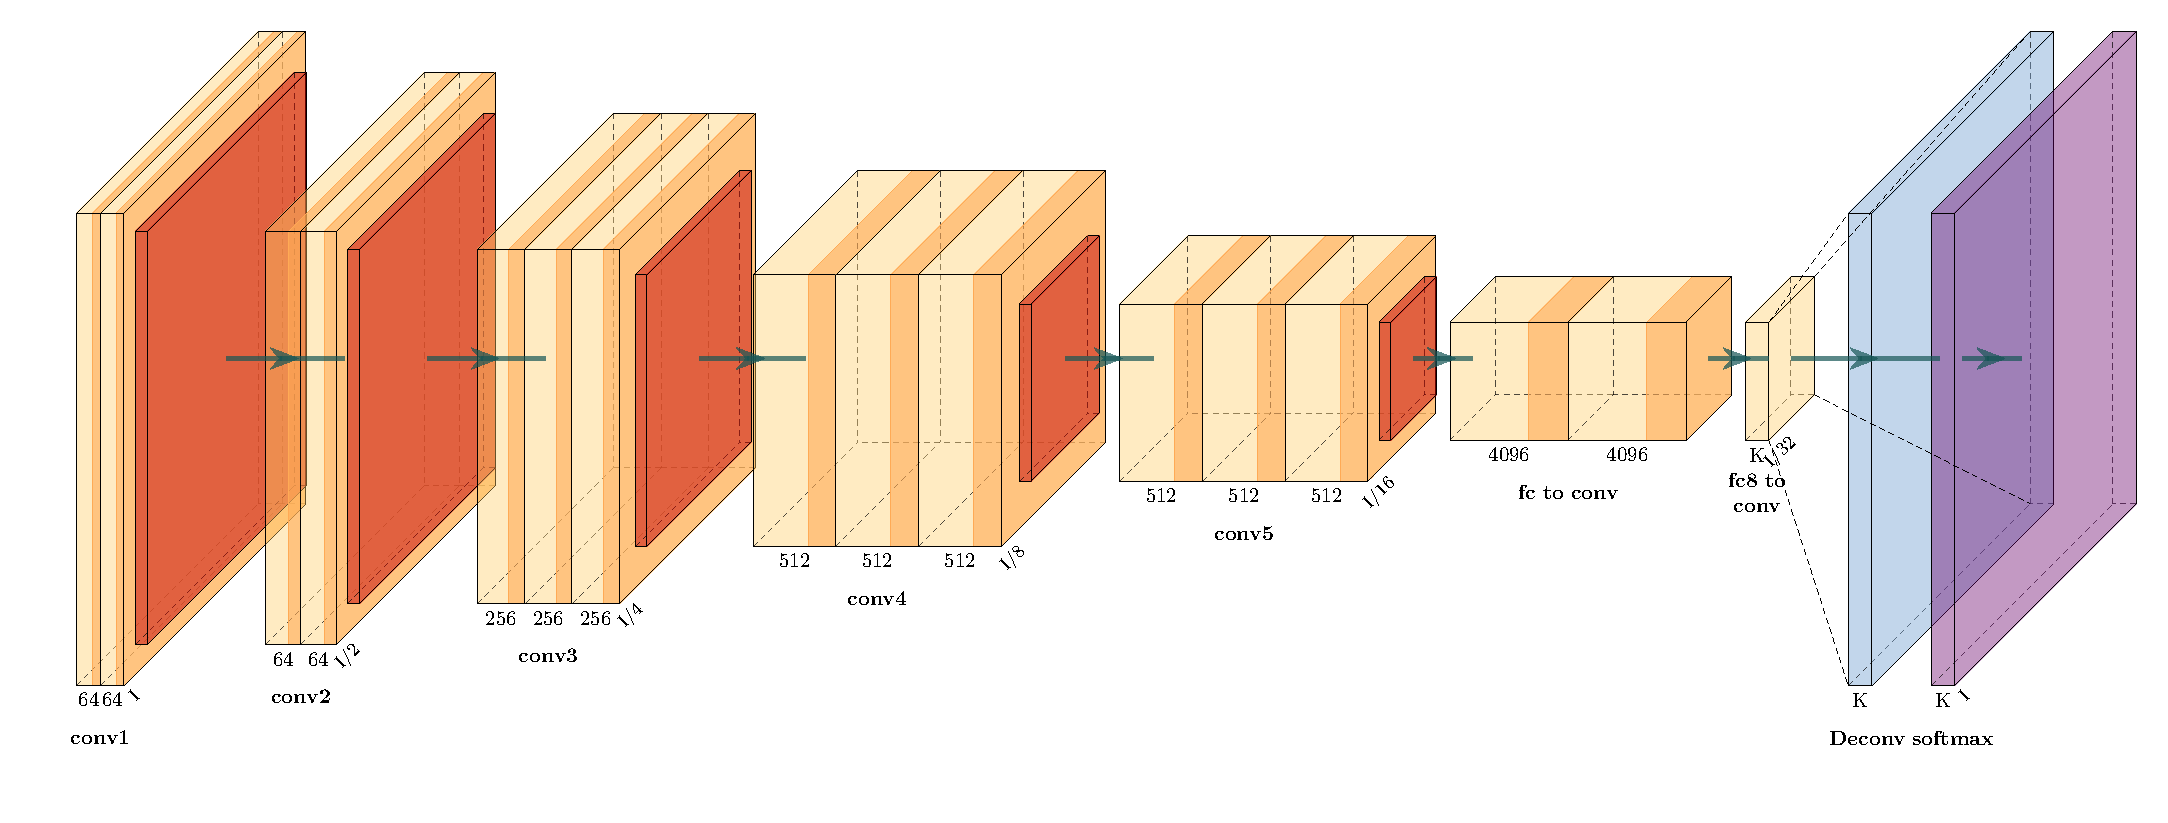
\includegraphics[width=\columnwidth]{picture/Structure/fcn.pdf}
%				%\captionsetup{font=scriptsize}
%				\caption{
%					\label{fig: fcn} 
%					Structure of feature fusion module.
%				}
%			\end{figure}
			
			\subsubsection{Approach}
			
			\begin{itemize}
				\item[(1)] 
				首先,将注意力机制引入到 ConvNeXt 骨干网络中,构造一个注意力 ConvNeX 模块(attention ConvNeX Module, ACM),然后对两个 ACM 模块进行堆叠。
				
				\item[(2)]
				其次,受 SKNet(Selective Kernel Networks) 和 CBAM (Convolutional Block Attention Module) 的启发,采用改进的混合注意机制 SKAM (Selective Kernel Attention Module)。该模块配置在两个堆叠的 ACM 之间,以实现感受野的自适应调节。该方法在有效抑制噪声的同时,提高了光照评价和细节恢复能力。
				
				\item[(3)]
				第三,充分融合不同层的特征,即浅层特征和深层特征,保留颜色信息,恢复纹理细节。
			\end{itemize}				
			
			\subsubsection{Future}
			
			-
			
		\subsection{(2019.4)Low-Light Image Enhancement via a Deep Hybrid Network}
		
		\paragraph{基于深度混合网络的弱光图像增强}
		
		\paragraph{(IEEE Transactions on Image Processing 1区) doi: 10.1109/TIP.2019.2910412}
		
			\subsubsection{Research Background}
			
			旨在弥补现有的弱光增强模型在结构细节上有所丢失的缺陷;
			
			\subsubsection{Contribution}

			为了保持图像的自然度并产生更准确的增强结果,提出了一种基于混合神经网络的弱光图像自动增强方法。网络由两个不同的流组成,在一个统一的网络中同时学习全局内容和清晰图像的显著结构。此外作者提出了一种新的空间变循环神经网络作为边缘流,在另一个自编码器的指导下对边缘细节进行建模,因为内容流中的编码器往往会丢失一些结构细节。
			
			\begin{figure}[htbp]
				% read manual to see what [ht] means and for other possible options
				\centering 
				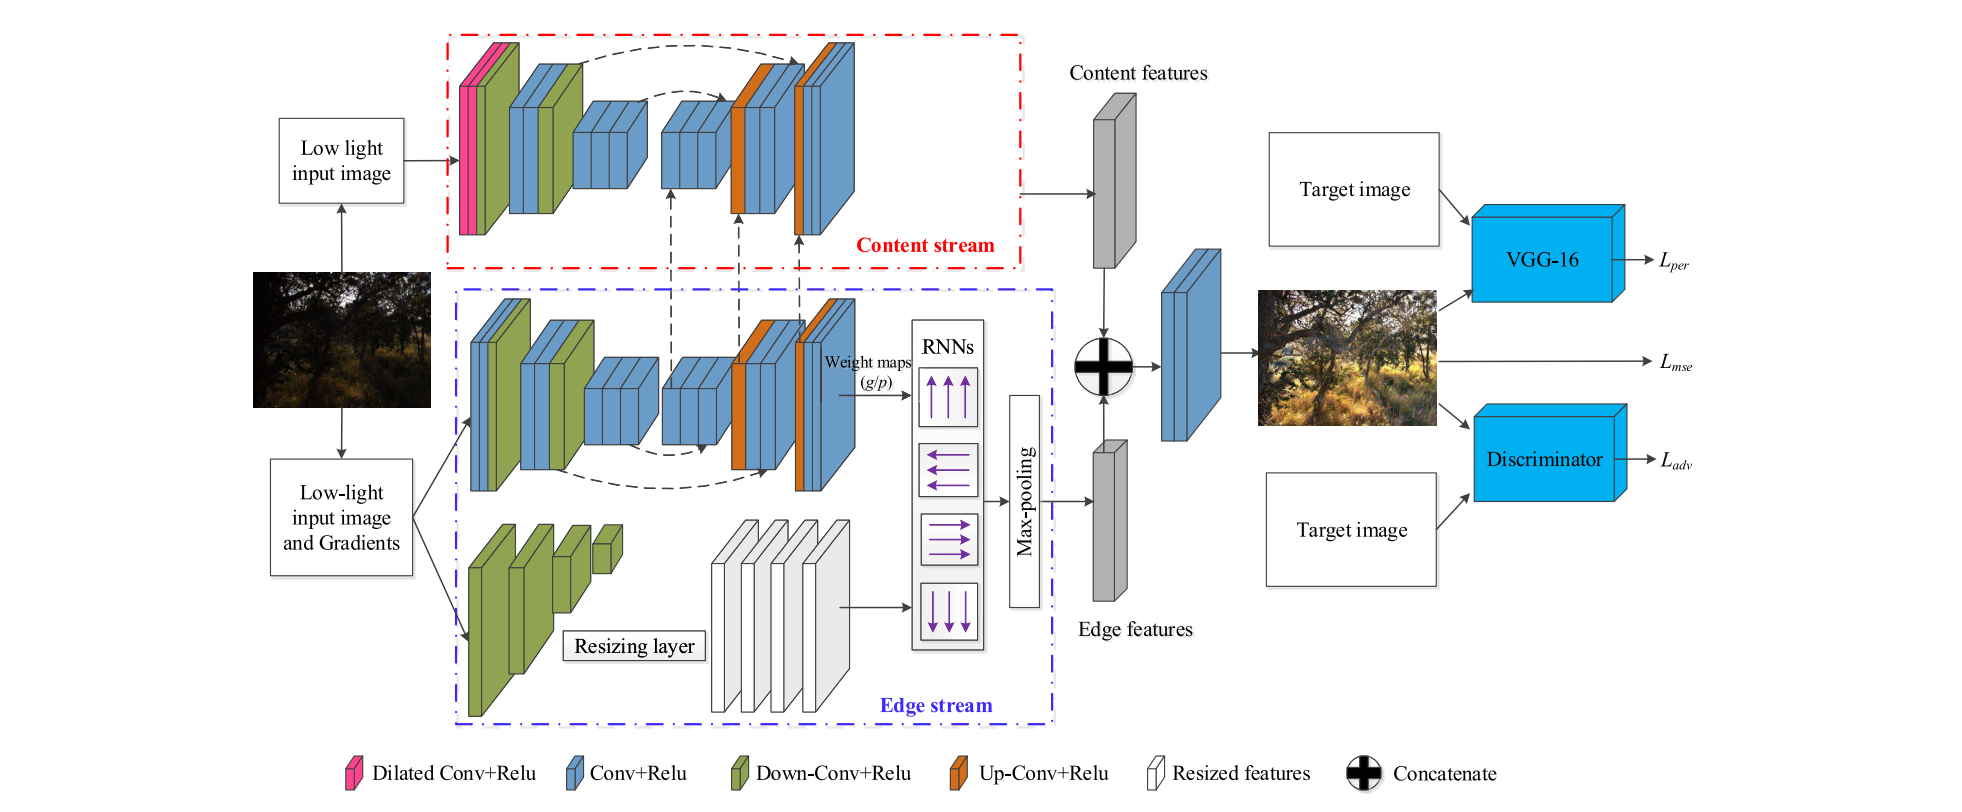
\includegraphics[width=\columnwidth]{picture/LLIE/DHN/Architecture}
				%\captionsetup{font=scriptsize}
				\caption{
					\label{fig: DHN Architecture} 
					Proposed low-light image enhancement architecture. Our model consists of two streams, the top content stream is a residual encoder-decoder which aims to restore most of the scene. The bottom edge stream focuses on the salient edge prediction via spatially variant RNNs. To construct communications between two streams, we bridge two networks during the up-sampling stage. In addition to the MSE loss function, we also adopt the perceptual and adversarial
					losses to further improve the visual quality.
				}
			\end{figure}
			
			具体的贡献如下:
			
			\begin{itemize}
				\item[(1)] 
				作者提出了一种混合神经网络,其中内容流用于预测输入的场景信息,边缘流用于边缘细节学习。所设计的网络能够更准确地恢复场景内容。
				
				\item[(2)]
				作者通过引入两个独立的权重映射作为 RNN 的输入特征和隐藏状态,提出了一种空间变异 RNN。RNN 对图像的内部结构(如边缘)进行建模,这在弱光图像增强中起着重要作用。
				
				\item[(3)]
				作者用感知损失和对抗损失训练混合网络,生成视觉上令人愉悦的增强图像,这些图像的表现优于最先进的方法。
			\end{itemize}	
			
			\subsubsection{Approach}
			
			\begin{itemize}
				\item[(1)] 
				作者通过由编码器和解码器组成的内容流来照亮输入图像,其中编码器用于捕获低光输入的上下文,解码器用于使用从编码器学习的表示来估计大部分场景。
				
				\item[(2)]
				由于内容流中的编码器网络丢失了一些图像细节,我们提出了一种边缘流网络,通过结合空间变异RNN,结合边缘感知特征映射并预测准确的图像结构。
				
				\item[(3)]
				由于增加细节的对比度可能会使噪声更明显,作者通过在训练数据中添加少量高斯噪声来缓解这个问题。
				
				\item[(4)]
				作者进一步结合了感知损失和对抗性损失,以提高增强结果的视觉质量。
				
			\end{itemize}	
		
			\paragraph{Edge Stream}
			
			作者采用以下方式来提取边缘信息;
			
			\begin{equation}
				\begin{aligned}
					h \left[k\right] = g \left[k\right] \circ x \left[k\right] + p \left[k\right] \circ h \left[k-1\right]
				\end{aligned}
				\label{eq: max and avg}
			\end{equation}
			
		 	其中 $h$ 为所求结构, $g, p$为权重参数,$x$ 为图像元素,$k$ 表示位置;总体上来说,$h\left[k\right]$ 上包含有图像在 $k$ 位置 $x\left[k\right]$ 的信息,还包含有上一个位置的边缘信息 $h\left[k-1\right]$,这两者的所占比重受权重 $g\left[k\right]$ 和 $p\left[k\right]$ 控制;而 $g, p$ 是未知的,因此作者采用可学习的 $g, p$ 来协助提取边缘信息;
		 	
		 	Edge Stream 部分是整篇论文的主要说明部分,也是其亮点之处;Edge Stream 也包含一个 Encode-Deconde 结构,该结构旨在求解出 $g, h$;而 Edge Stream 下方的结构为 downsampling + conv 和 resize 的操作;把 input image 分别下采样到 $\frac{1}{2}, \frac{1}{4}, \frac{1}{8}$,然后进行一次卷积操作;然后再将 $\frac{1}{2}, \frac{1}{4}, \frac{1}{8}$ 大小的 map resize 到和原来的大小一致。然后分别从 $left \rightarrow right$,$right \rightarrow left$,$up \rightarrow down$,$down \rightarrow up$ 四个方向根据上面提到的公式来得出各方向上的 $h$,最后用每个 $k$ 位置的四个方向的 $h\left[k\right]$ 的最大值来作为 $k$ 位置的边缘隐藏信息(即Fig .\ref{fig: DHN Architecture}中的 Max-pooling );

			\subsubsection{Future}
			
			-
			
		\subsection{(2023.5)A Fusion-Based and Multi-Layer Method for Low Light Image Enhancement}
	
		\paragraph{基于深度混合网络的弱光图像增强}
	
		\paragraph{(ICASSP 2023) doi: 10.1109/ICASSP49357.2023.10096454}
		
			\subsubsection{Research Background}
			
			目前许多弱光图像算法的增强效果不自然,对比度不足。以往的算法将弱光图像的照度划分为多层低频分量,进行校正后达到正常照度范围。但仅对照度进行粗暴的校正不能在亮度增强和对比度增强之间取得良好的平衡。
			
			\subsubsection{Contribution}
			
			作者将输入图像的照度分解为高频和低频分量。然后,基于先验统计,使用两种不同的校正函数对光照进行调整,并对其进行迭代分解,直到最终分布均匀。最后,将所有分解后的反射率与最后一层校正后的照度相乘,得到增强结果。
			
			\begin{itemize}
				\item[(1)] 
				作者提出了一种基于融合的增强和多层模型相结合的方法。
				
				\item[(2)]
				作者创新地提出两种照明校正功能,有效地保持了校正后的照明结构。
				
				\item[(3)]
				作者设计了一条新的拟合曲线,通过在先验亮度统计中加入标准方差和校正函数来提高性能。
			\end{itemize}	
			
			\subsubsection{Approach}
			
			\begin{figure}[htbp]
				% read manual to see what [ht] means and for other possible options
				\centering 
				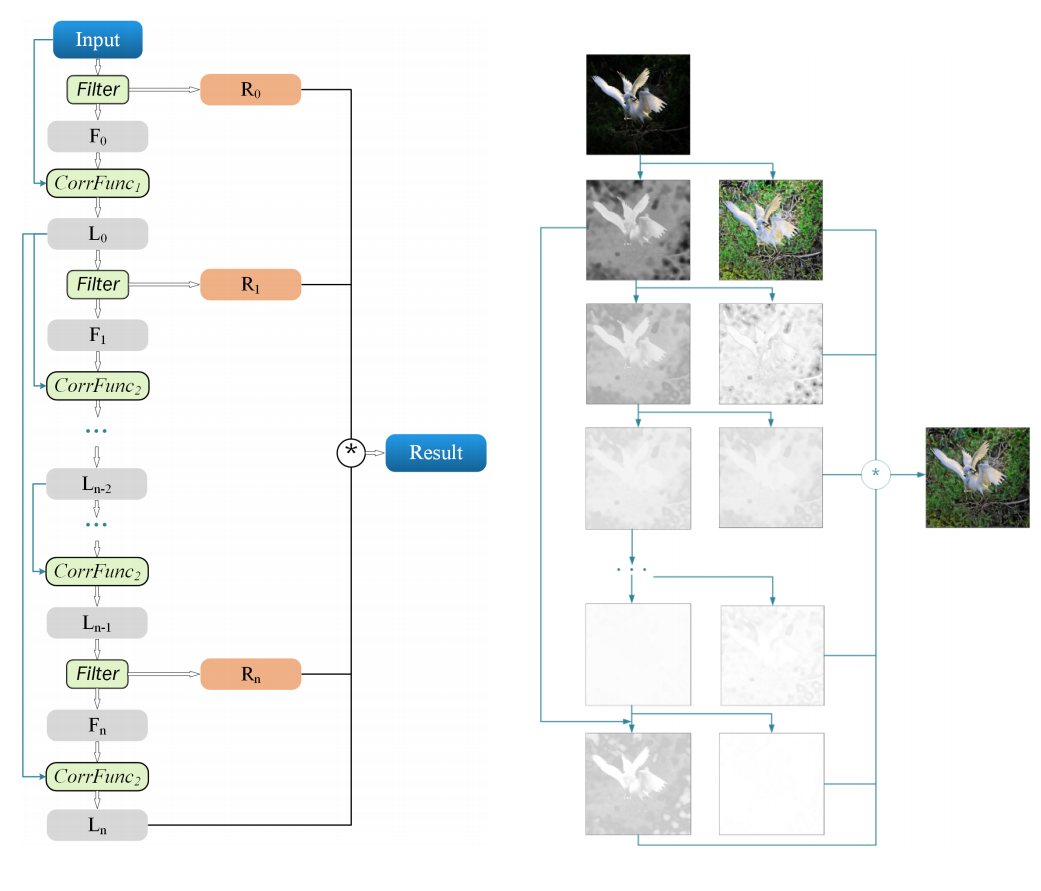
\includegraphics[width=0.7\columnwidth]{picture/LLIE/Fusion-based/decomposition and enhancement}
				%\captionsetup{font=scriptsize}
				\caption{
					\label{fig: decomposition and enhancement} 
					Image decomposition and enhancement using the multi-layer model.
				}
			\end{figure}
			
			\begin{itemize}
				\item[(1)] 
				首先,基于 HSV 空间\footnote{HSV 颜色空间是一种颜色模型,由 A.R.Smith 在 1978 年提出,也被称为六角锥体模型。HSV 颜色空间的三个参数分别是:
					\begin{itemize}
						\item[$\bullet$] 
						色调 (Hue): 用角度度量,取值范围为 $0^{\circ} \sim 360^{\circ}$,表示色彩信息,即所处的光谱颜色的位置。例如,红色为 $0^{\circ}$,绿色为 $120^{\circ}$,蓝色为 $240^{\circ}$ 等等。
						
						\item[$\bullet$]
						饱和度 (Saturation): 取值范围为 $0.0 \sim 1.0$。饱和度表示颜色接近光谱色的程度。饱和度越高,说明颜色越深,越接近光谱色。饱和度越低,说明颜色越浅,越接近白色。
						
						\item[$\bullet$]
						明度 (Value): 取值范围为 $0.0 (black) \sim 1.0 (white)$。明度决定了颜色的明亮程度。
					\end{itemize}
					
					HSV 颜色空间相比于 RGB 颜色空间更加直观,更接近人们对彩色的感知经验。在图像处理中,HSV 颜色空间常用于分割指定颜色的物体。}从弱光图像中获取 $V$ 通道,并利用低通滤波器将其分解为低频和高频分量;低频分量可以导出两个输入分量。
				
				\item[(2)]
				其次,利用基于先验统计量的校正函数融合两个输入,得到当前层的输出;
				
				\item[(3)]
				第三,对得到的分量进行多次分解和融合迭代。
				
				\item[(4)]
				最后,作者将最后修正的低频分量与所有高频分量结合起来,形成最终结果。
				
			\end{itemize}	
			
			\subsubsection{Future}
			
			-
		
		\subsection{(2023.5)A Fusion-Based and Multi-Layer Method for Low Light Image Enhancement}
		
		\paragraph{基于模拟多曝光融合的弱光图像增强}
		
		\paragraph{(Journal of Physics: Conference Series 4区) doi: 10.1088/1742-6596/2478/6/062022}
		
			\subsubsection{Research Background}
			
			目前的方法可以获得具有良好人类视觉感知的增强图像,但这些结果可能会受到局部对比度低和细节模糊的影响,特别是在曝光不足的区域。在昏暗环境中拍摄的单幅图像中,对比度和细节增强有待提升。
			
			\subsubsection{Contribution}
			
			作者提出了一种结合增强算法和曝光融合技术优点的新颖有效的框架。
			
			受曝光融合技术的启发,作者采用模拟多曝光图像融合技术,在光照不足或不均匀、背光和曝光时间有限等恶劣条件下拍摄图像,获得明亮、自然和令人满意的结果。
			
			\subsubsection{Approach}
			
			作者设计了一种新的方法,从单幅图像生成不同曝光时间的合成图像。因此,这些人工序列的每个图像都包含最终所需增强结果的必要信息。然后,作者引入了一个灵活的多曝光融合框架来实现融合图像,该框架包括权重图预测模块和多尺度融合模块。
						
			曝光融合是一种高效的高动态范围 (HDR) 融合技术,其关键在于从每幅低动态范围 (LDR) 图像中融合出曝光良好的像素。受这个想法的启发,作者将退化图像本身的良好感知区域合并为高质量的增强图像。
			
			作者提出的方法共分为两个阶段(如 Fig. \ref{fig: Schematic diagram} 所示)
			
			\begin{itemize}
				\item[(1)] 
				作者的方法的第一阶段是生成一个人工图像序列。这些合成图像分别包含几个曝光良好的区域,这些地图并不完全一致。换句话说,每个仿真图像集中在原始图像的不同区域,不同的显著区域构成了整个图像。
				
				\item[(2)]
				下一阶段是合并这些人工曝光序列。提出了一种改进的多尺度融合方法,以更好地融合序列并保留颜色信息。
			\end{itemize}	
			
			\begin{figure}[htbp]
				% read manual to see what [ht] means and for other possible options
				\centering 
				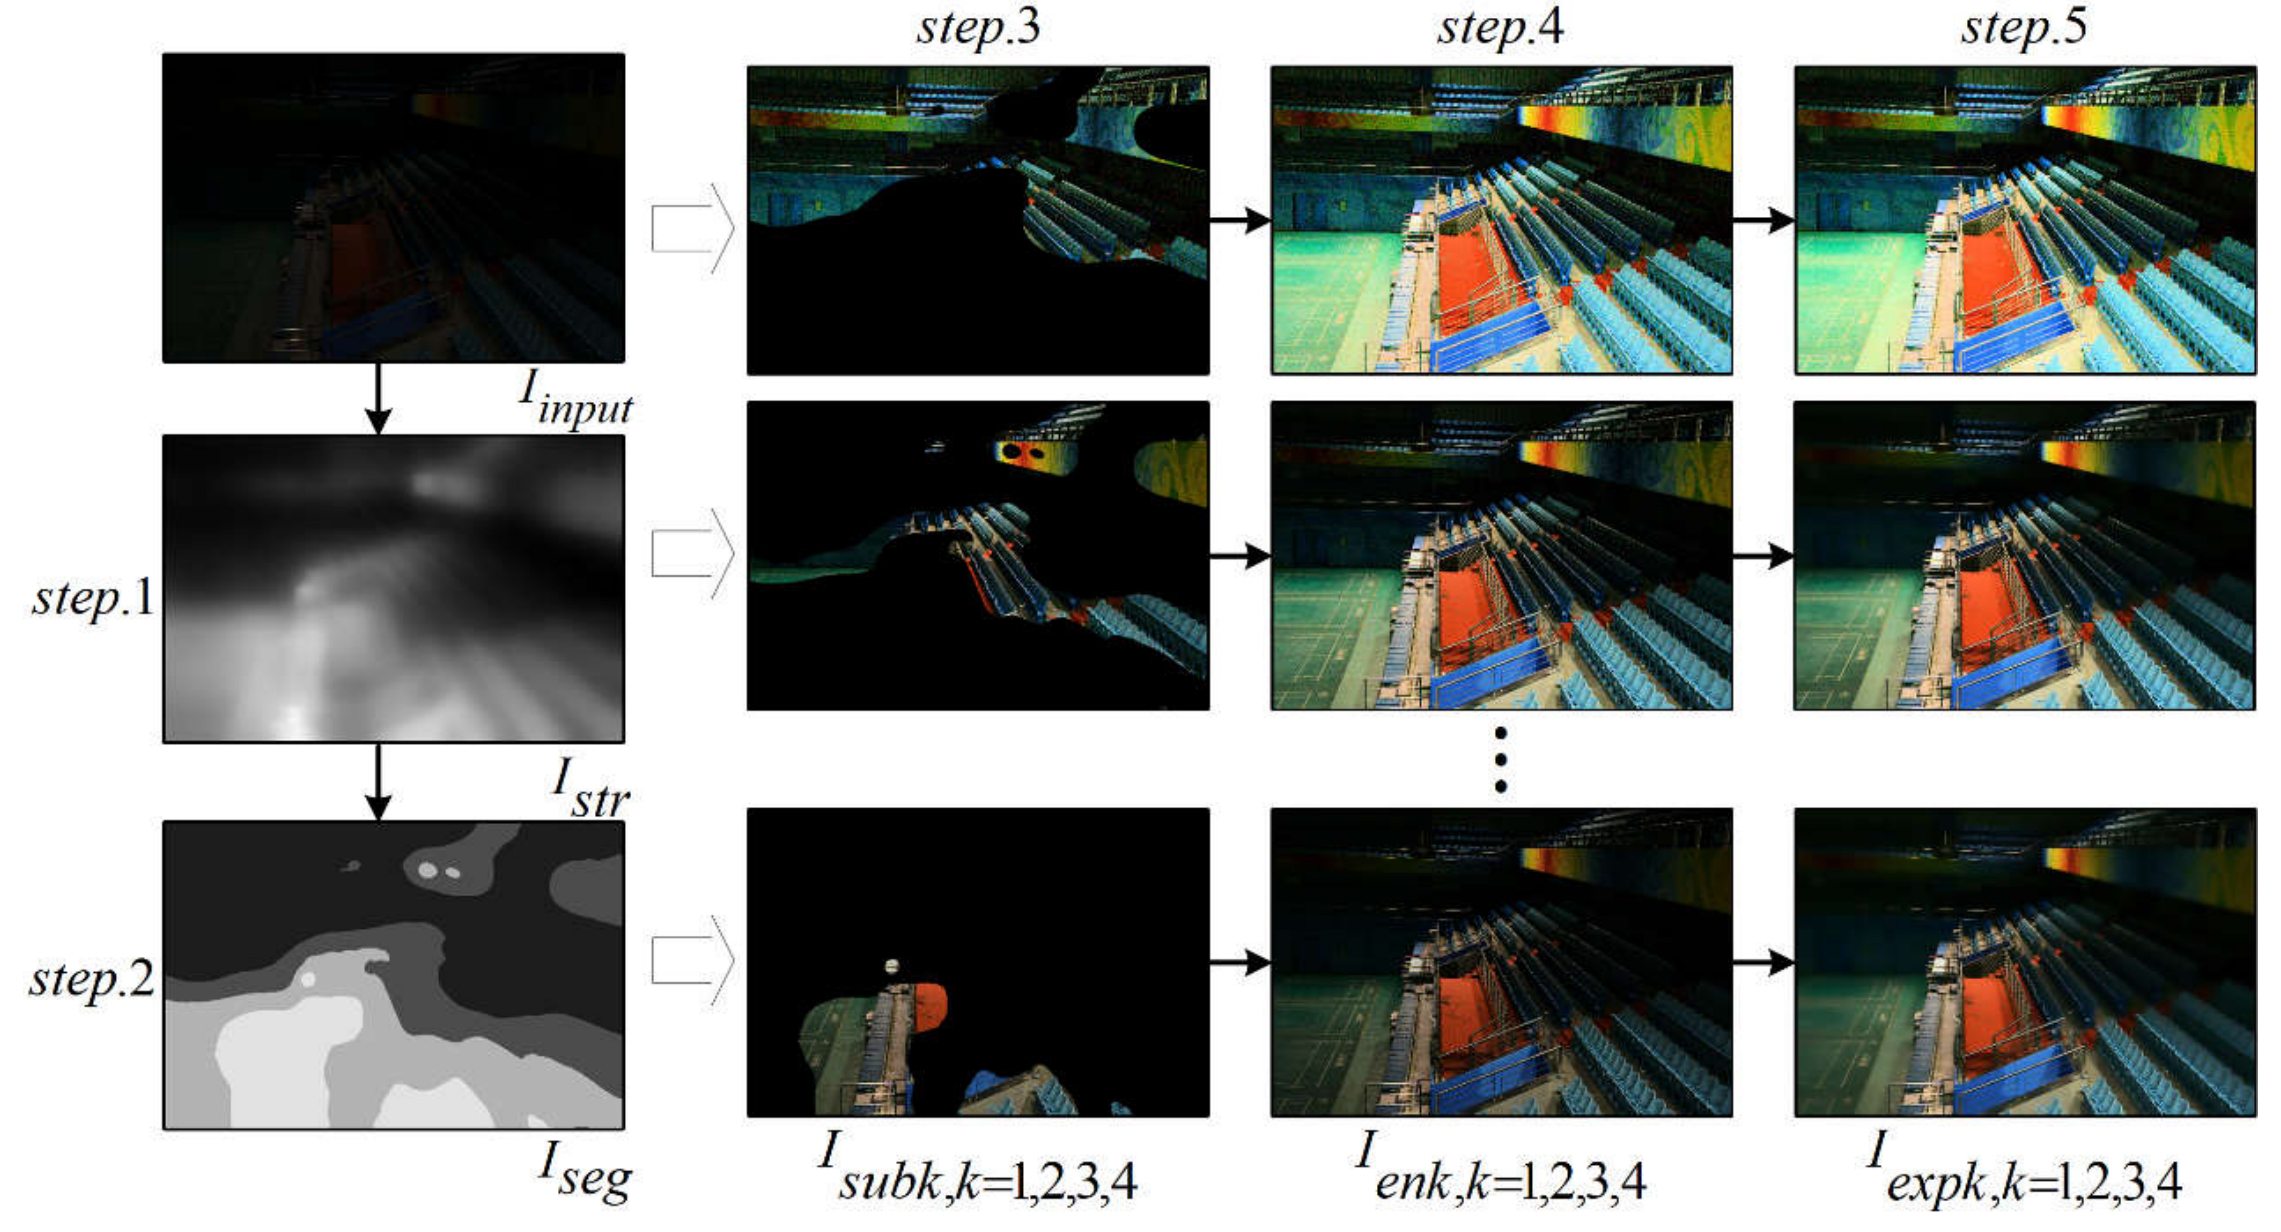
\includegraphics[width=\columnwidth]{picture/LLIE/Multi-exposure fusion/Schematic diagram}
				%\captionsetup{font=scriptsize}
				\caption{
					\label{fig: Schematic diagram} 
					Schematic diagram of the simulated exposure sequence generation method. For the sake of observation, $I_{subk}$ are the enhanced results of $I_{input-subk}$.
					}
			\end{figure}
			
			\subsubsection{Future}
			
			-
			
		\subsection{(2023.3)Fusion-Based Low-Light Image Enhancement}
		
		\paragraph{基于模拟多曝光融合的弱光图像增强}
		
		\paragraph{(International Conference on Multimedia Modeling C类) doi: 10.1088/1742-6596/2478/6/062022}
		
			\subsubsection{Research Background}
			
			除了对比度差之外,在光线不足的情况下拍摄的图像还会受到严重的噪声和饱和度失真的影响。现有的基于无监督学习的方法大多采用两阶段处理的方法,依次增强对比度和去噪。但是,在对比度增强过程中,噪声会被放大,从而增加去噪的难度。此外,现有的无监督弱光增强方法没有很好地考虑光照不足引起的饱和畸变。
			
			\subsubsection{Contribution}
			
			作者提出了一种新的并行框架,该框架包括饱和度自适应调整分支、亮度调整分支、噪声抑制分支以及分别用于调整饱和度、校正亮度、去噪和多分支融合的融合模块。
			
			作者贡献总结如下:
			
			\begin{itemize}
				\item[(1)] 
				提出了一种并行融合框架,可同时进行对比度增强、饱和度校正和去噪。整个框架以无监督的方式进行训练。
				
				\item[(2)]
				提出了一种基于灰色世界算法和 Von Kries 对角模型的饱和度自适应校正方法。
				
				\item[(3)]
				在多分支融合中引入可训练的无监督引导滤波融合模块,进一步抑制噪声。
								
			\end{itemize}	
			
			\subsubsection{Approach}
			
			作者提出的并行框架如 Fig. \ref{fig: Parallel fusion frame diagram} 所示,该框架由三个主要分支和一个融合模块组成,输入图像在融合前分别通过亮度和饱和度校正和去噪声并行增强。将输入图像从 RGB 色彩空间转换为 HSV 色彩空间,并分别通过饱和度和亮度校正分支对 S 和 V 通道进行校正。同时,噪声抑制分支在 RGB 色彩空间上对输入图像并行进行初步去噪。最后,各支路的输出通过融合模块进行融合。
			
			\begin{figure}[htbp]
				% read manual to see what [ht] means and for other possible options
				\centering 
				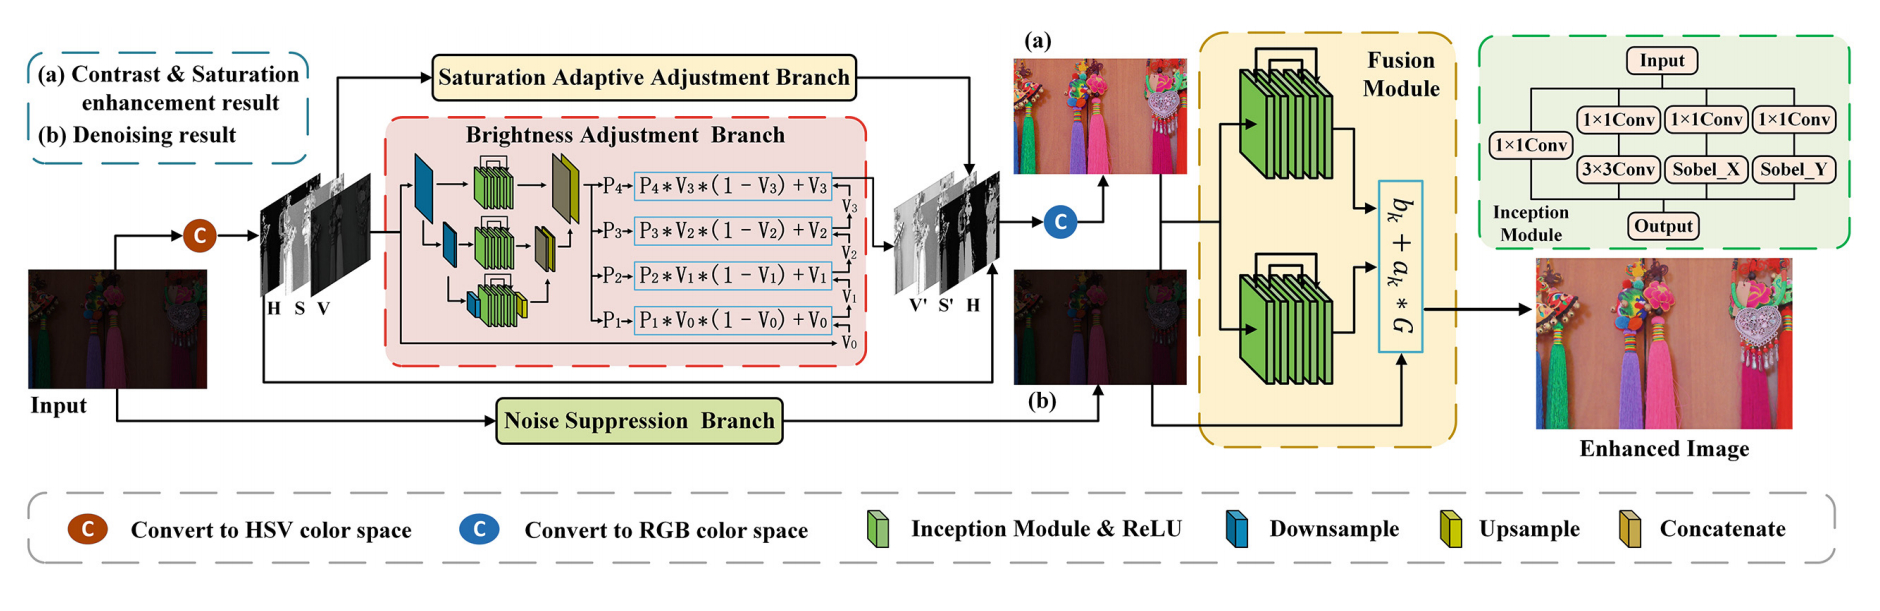
\includegraphics[width=\columnwidth]{picture/LLIE/Fusion-Based LLIE/Parallel fusion frame diagram}
				%\captionsetup{font=scriptsize}
				\caption{
					\label{fig: Parallel fusion frame diagram} 
					Parallel fusion frame diagram, where the red box represents the brightness adjustment branch, and the green box represents the inception module. 
				}
			\end{figure}
			
		\subsection{(2022.12)Dual UNet low-light image enhancement network based on attention mechanism}
		
		\paragraph{基于模拟多曝光融合的弱光图像增强}
		
		\paragraph{(Multimedia Tools and Applications 4区)}
		
			\subsubsection{Research Background}
			
			U-Net 网络在弱光图像增强方面显示出更好的前景。然而,由于 U-Net 网络中的语义缺口和全局上下文信息之间缺乏联系,导致增强图像中的颜色信息不准确等问题。
			
			\subsubsection{Contribution}
			
			作者为了克服 U-Net 网络在弱光图像增强方面的局限性,提出了一种基于注意机制的双 U-Net 微光图像增强网络 (DUAMNet)。
			
			主要的贡献有以下几点:
			
			\begin{itemize}
				\item[(1)] 
				作者提出了一种新的基于双 U-Net 的低光图像增强网络。AU-Net++ 网络旨在克服基于 U-Net 网络的弱光图像增强网络的两个局限性。结合 U-Net 和 AU-Net++ 组成我们的亮度增强模块 (BEM), BEM 从多尺度的角度捕捉不同层次的特征,增强不同层次信息之间的联系,从各个方向学习图像特征信息。
				
				\item[(2)]
				CBAM 调用 AU-Net++ 中的轻量级双注意机制 CBAM,进一步加强了 U-Net++ 与全局上下文信息建立联系的能力,同时 CBAM 在通道和空间两个维度上关注特征信息,使网络更有效地关注复杂融合特征中的低光区域。
				
				\item[(3)]
				采用局部二值模式算子 (LBP) 作为图像纹理特征提取器,利用 LBP 算法的光照不变性有效描述图像的微观结构信息。在网络的每个递归阶段提取图像的纹理特征,有效地提高了网络的特征表达能力。
				
				\item[(4)]
				网络框架采用递进递归结构。每一阶段的输入就是前一阶段的输出,将前一阶段的特征信息作为先验特征信息来指导当前递归阶段的特征学习。递归结构有效地整合了各阶段的特征信息。增强的网络建模功能。
				
			\end{itemize}	
			
			\begin{figure}[htbp]
				% read manual to see what [ht] means and for other possible options
				\centering 
				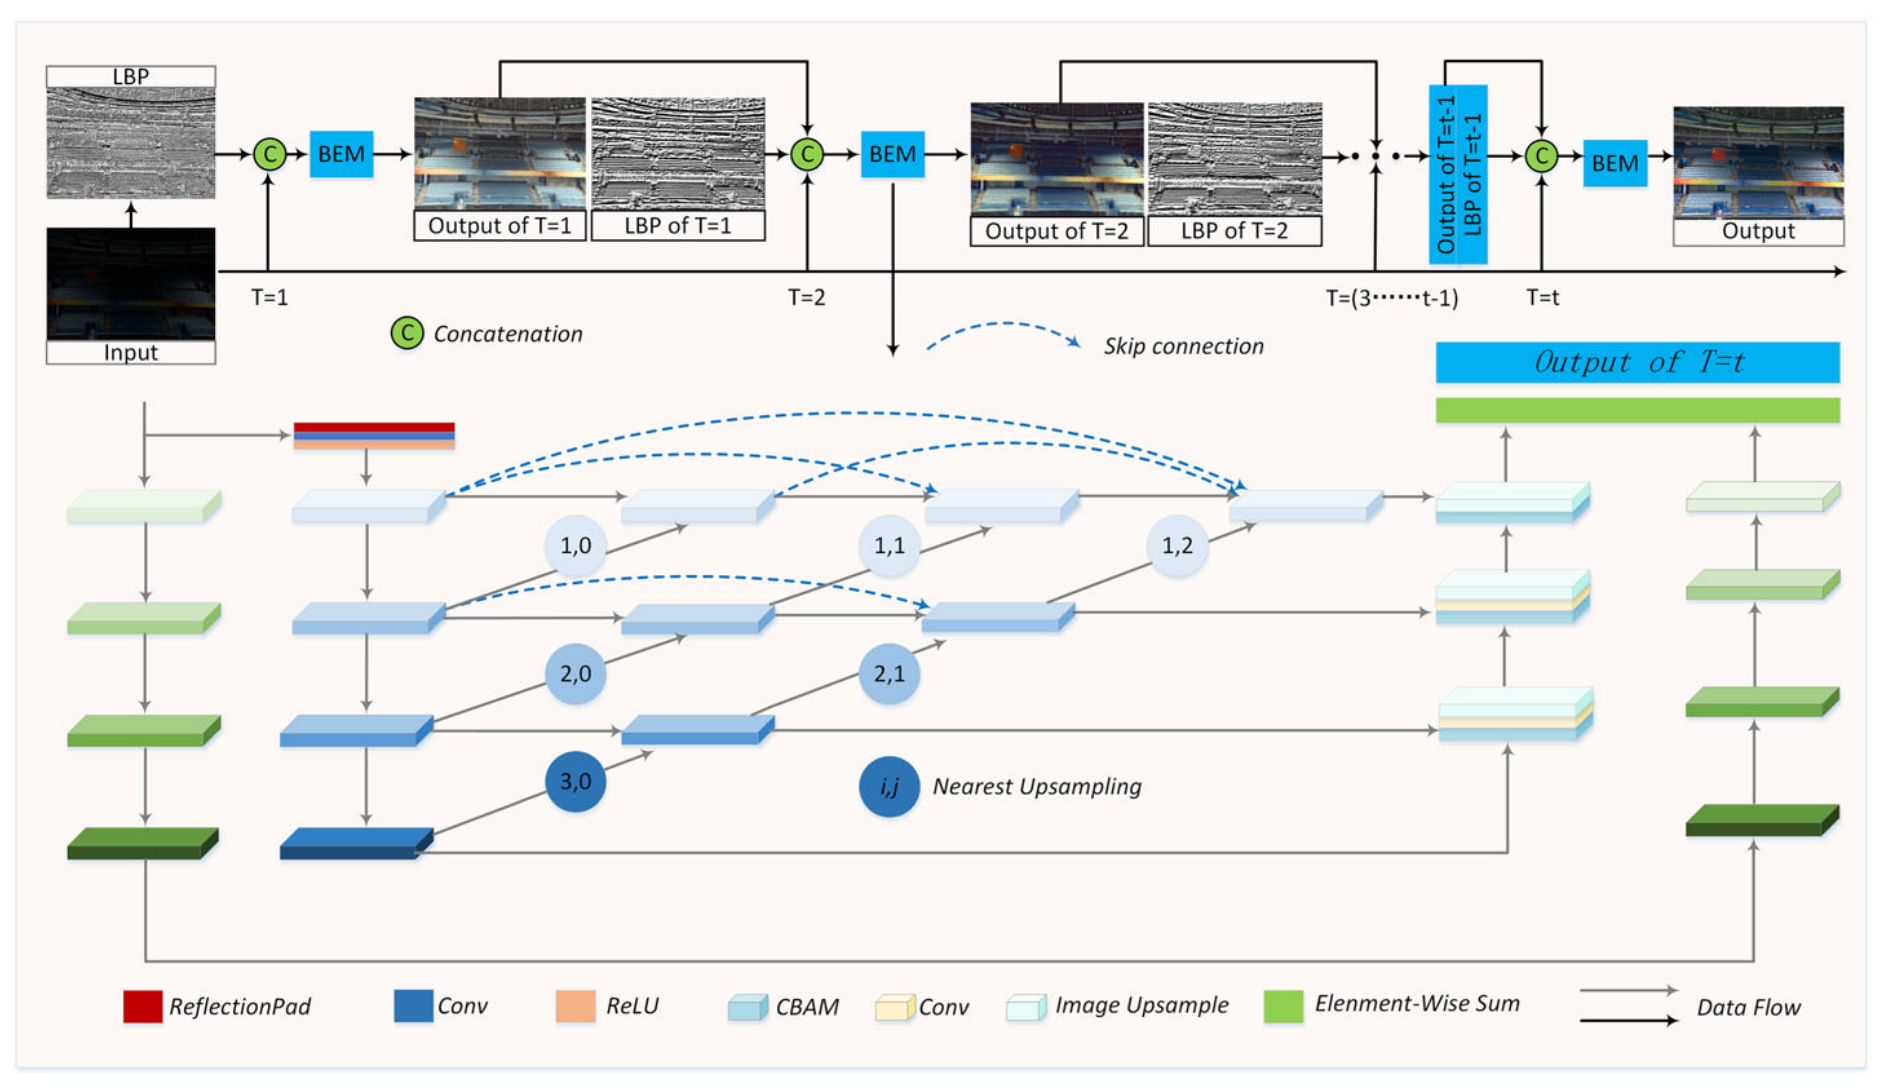
\includegraphics[width=\columnwidth]{picture/LLIE/Dual UNet/DUAMNet framework}
				%\captionsetup{font=scriptsize}
				\caption{
					\label{fig: DUAMNet framework} 
					The framework of DUAMNet. The network is divided into T recursive stages
				}
			\end{figure}
			
			\subsubsection{Approach}
	
			\begin{itemize}
				\item[(1)] 
				首先,利用局部二值模式 (local Binary Pattern, LBP) 算子提取原始图像的局部纹理特征,LBP 算子的光照不变性较好地保持了原始图像的纹理信息;
				
				\item[(2)]
				接下来,使用亮度增强模块 (BEM)。在 BEM 模块中,外部 U-Net 网络捕获不同层次的特征信息和不同区域的亮度信息,内部密集连接的 U-Net++ 网络增强了不同层次特征信息的相关性,挖掘了编码器提取的更多隐藏特征信息,减少了编码器和解码器之间的特征语义差距。
				
				\item[(3)]
				在 U-Net++ 网络解码器中引入了卷积块注意模块 (CBAM)。CBAM 进一步增强了对全局上下文信息链接的建模能力,有效提高了网络对弱光区域的关注。网络采用递进递归结构。整个网络包括四个递归单元,前一个递归单元的输出作为下一个递归单元的输入。
				
				\item[(4)]
				在七个公共数据集上进行了对比实验,并对结果进行了定量和定性分析。结果表明,尽管本文网络结构简单,但与其他方法相比,本文网络在图像质量上优于其他方法。
				
			\end{itemize}	
		
			\subsubsection{Future}
			
			-
		
		\subsection{(2022.10)Effective low-light image enhancement with multiscale and context learning network}
		
		\paragraph{基于多尺度和上下文学习网络的有效弱光图像增强}
		
		\paragraph{(Multimedia Tools and Applications 4区)}
		
			\subsubsection{Research Background}
			
			卷积神经网络 (CNN) 在弱光图像增强任务中得到了广泛的应用,并取得了良好的增强效果。然而,增强结果不仅受到卷积核的限制,而且还受到弱光区域形状和大小的影响。CNN 只能捕获局部依赖关系。难以从图像中获得远距离依赖关系和多尺度特征,导致增强过或不足。
			
			\subsubsection{Contribution}
			
			作者提出了一种多尺度和上下文学习网络 (MCLNet),通过多尺度特征提取和全局关系学习来实现自适应弱光增强。
			
			MCLNet 的主要贡献如下:
			
			\begin{itemize}
				\item[(1)] 
				从局部和全局的角度,作者提出了一个多尺度和上下文学习网络 (MCLNet),用于多尺度表示学习和远程依赖建模的自适应弱光增强。
				
				\item[(2)]
				作者引入了一个带有残差学习和注意机制的多尺度学习块,称为 ARMB,来学习多尺度表示。在ARMB的基础上,引入的 BSAM 捕获有关全局和局部上下文的信息,使网络能够基于全局信息增强局部区域。
				
				\item[(3)]
				作者提出的 CEM 可以从不同弱光区域的多尺度信息中建模全局关系,从而增强自适应弱光增强能力。
				
			\end{itemize}	
			
			\subsubsection{Approach}
			
			\begin{figure}[htbp]
				% read manual to see what [ht] means and for other possible options
				\centering 
				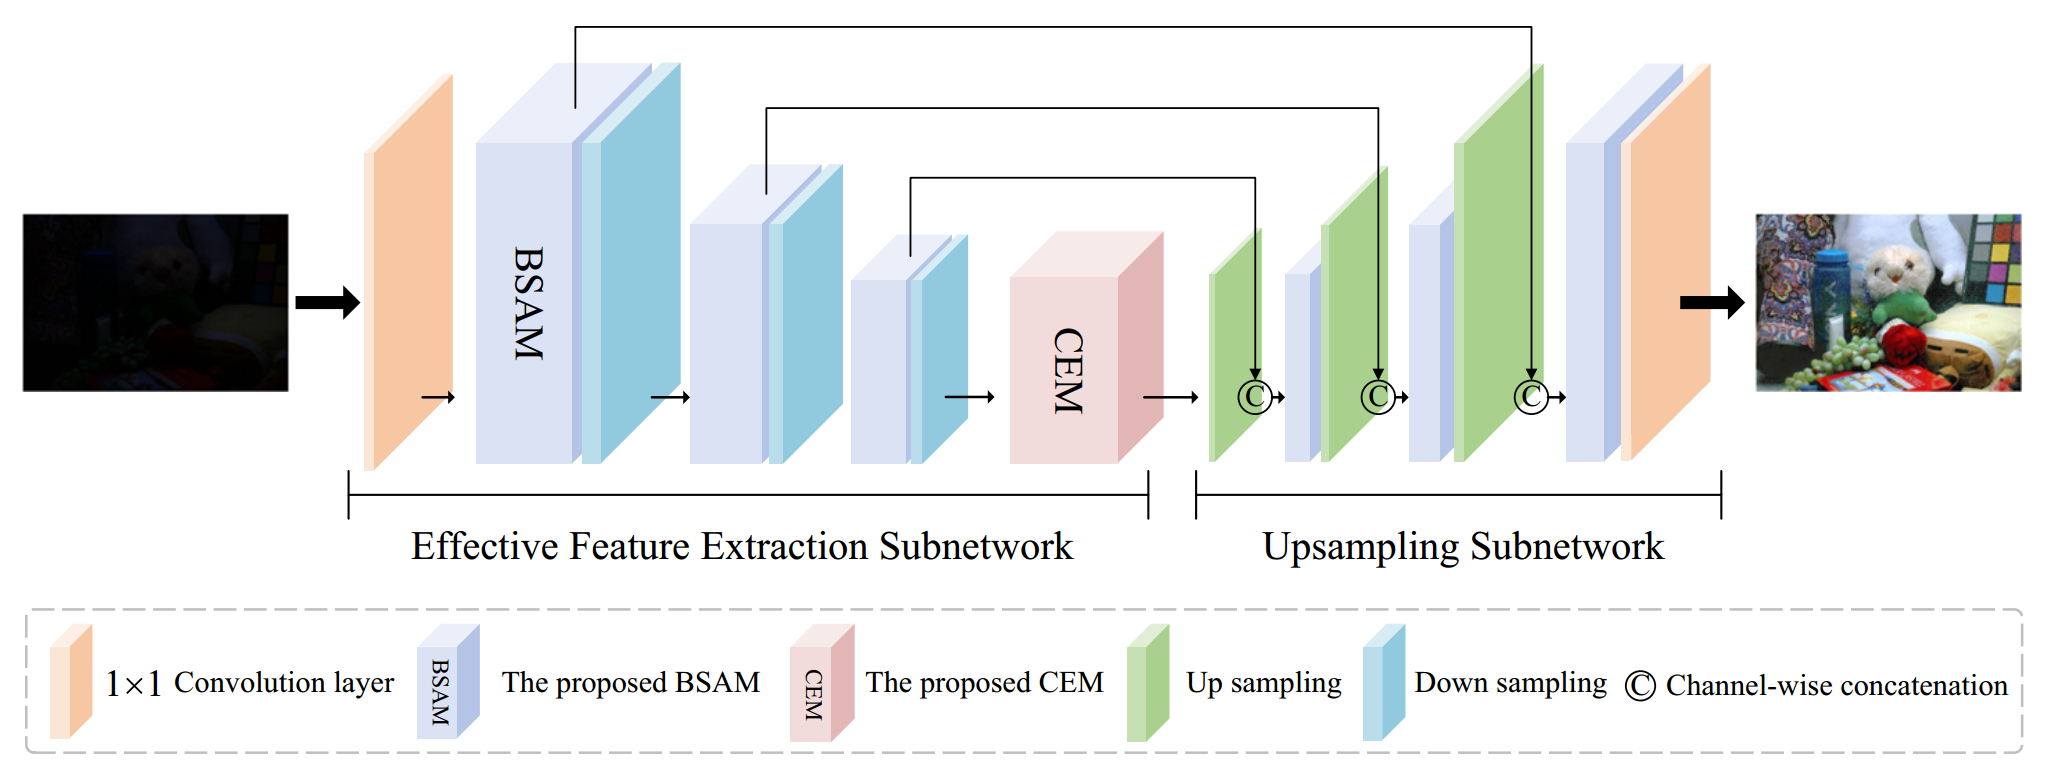
\includegraphics[width=\columnwidth]{picture/LLIE/MCLNet/Overview}
				%\captionsetup{font=scriptsize}
				\caption{
					\label{fig: MCLNet Overview} 
					Overview of Multiscale and Context Learning Network (MCLNet).
				}
			\end{figure}
			
			具体而言,为了获得不同低光区域的判别表征,作者设计了一个注意残差多尺度块 (ARMB),通过不同尺度的空间注意机制捕获有价值的多尺度特征。在此基础上,提出了一种规模聚合模块 (BSAM) 来学习分层判别特征。最后,为了进一步从全局角度进行自适应增强,作者提出了一个上下文编码模块 (CEM),通过 Transformer 对远程依赖进行建模。
			
			\begin{figure}[htbp]
				% read manual to see what [ht] means and for other possible options
				\centering 
				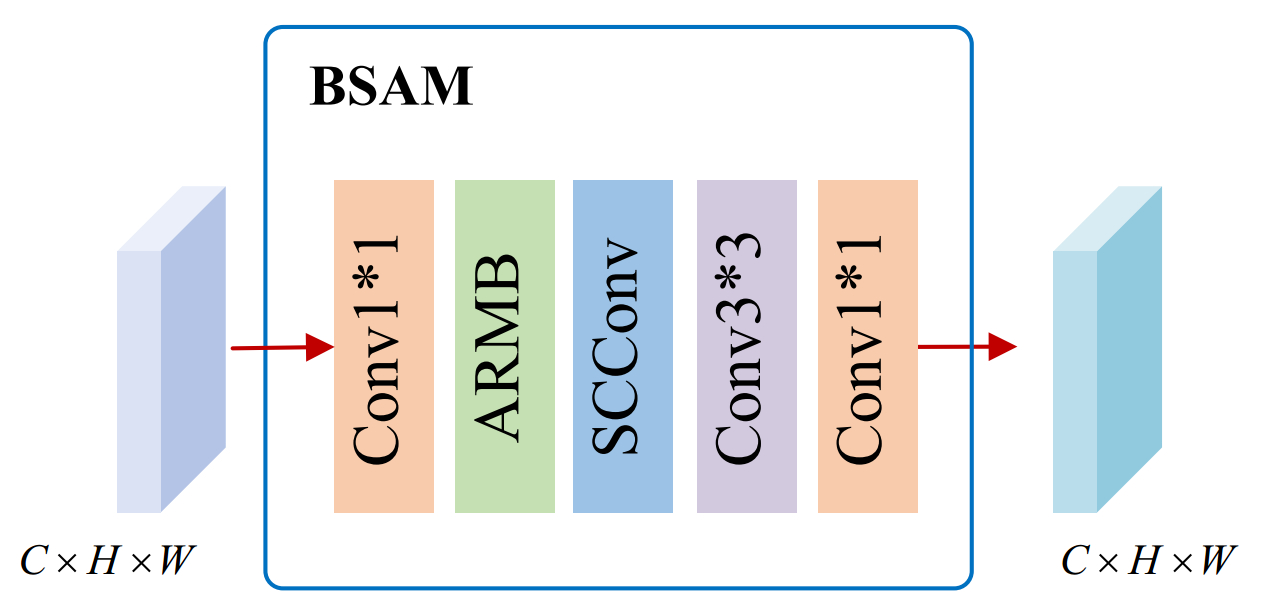
\includegraphics[width=0.7\columnwidth]{picture/LLIE/MCLNet/BSAM}
				%\captionsetup{font=scriptsize}
				\caption{
					\label{fig: MCLNet BSAM} 
					The architecture of the Bottleblock of Scale Aggregation module (BSAM)
				}
			\end{figure}
			
			\begin{figure}[htbp]
				% read manual to see what [ht] means and for other possible options
				\centering 
				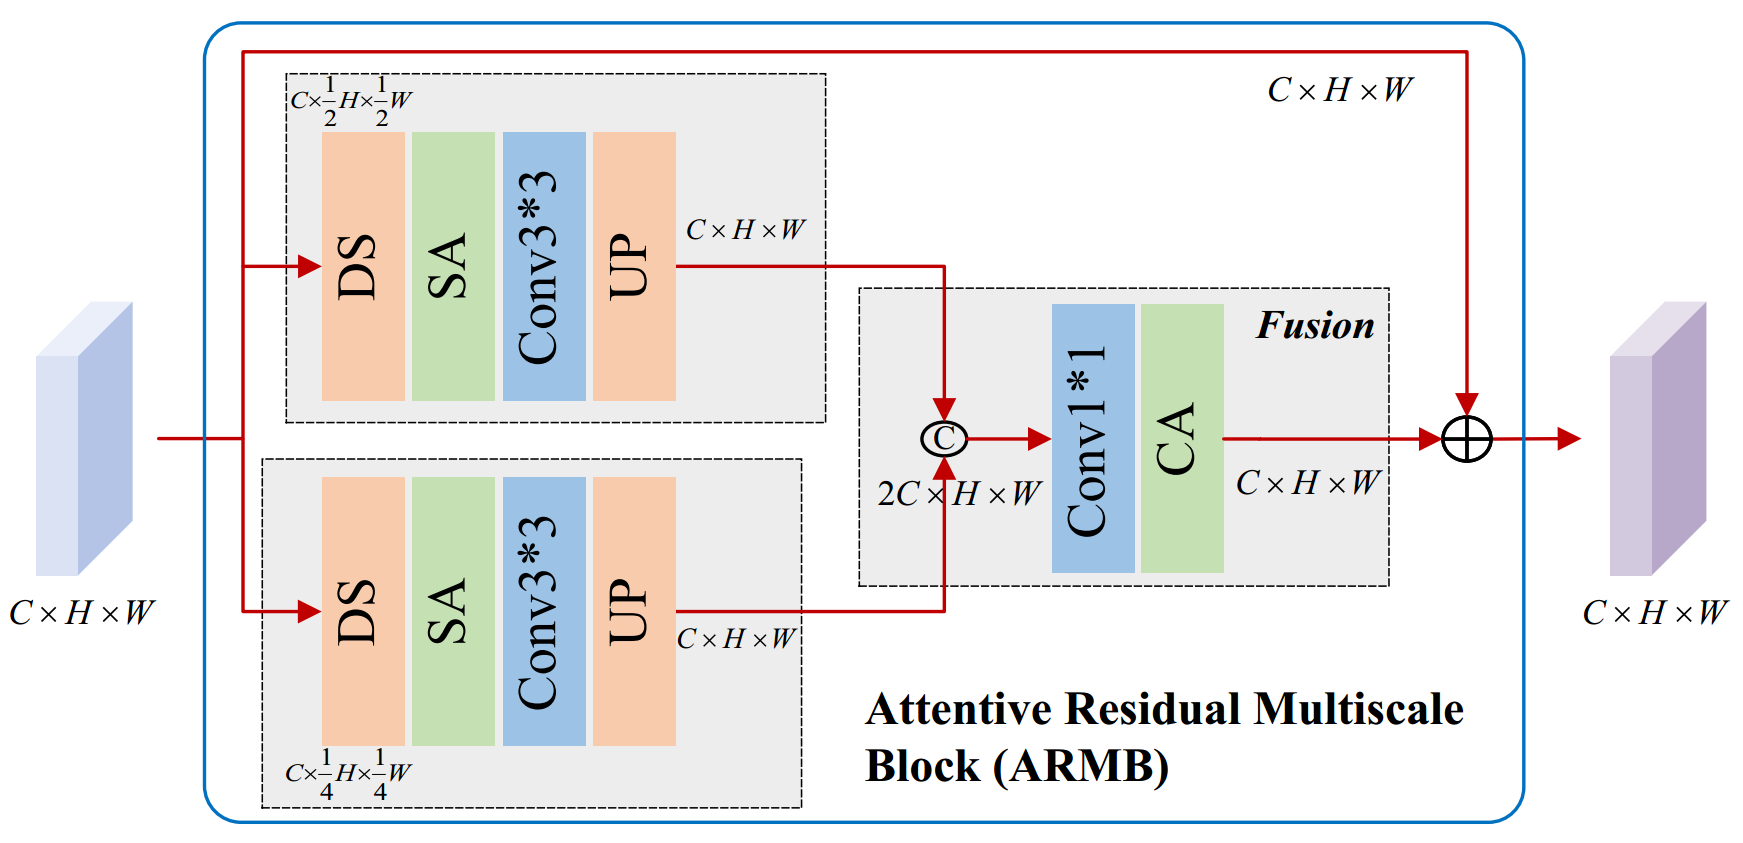
\includegraphics[width=0.7\columnwidth]{picture/LLIE/MCLNet/ARMB}
				%\captionsetup{font=scriptsize}
				\caption{
					\label{fig: MCLNet ARMB} 
					The architecture of the Attentive Residual Multiscale Block (ARMB)
				}
			\end{figure}
			
			\begin{figure}[htbp]
				% read manual to see what [ht] means and for other possible options
				\centering 
				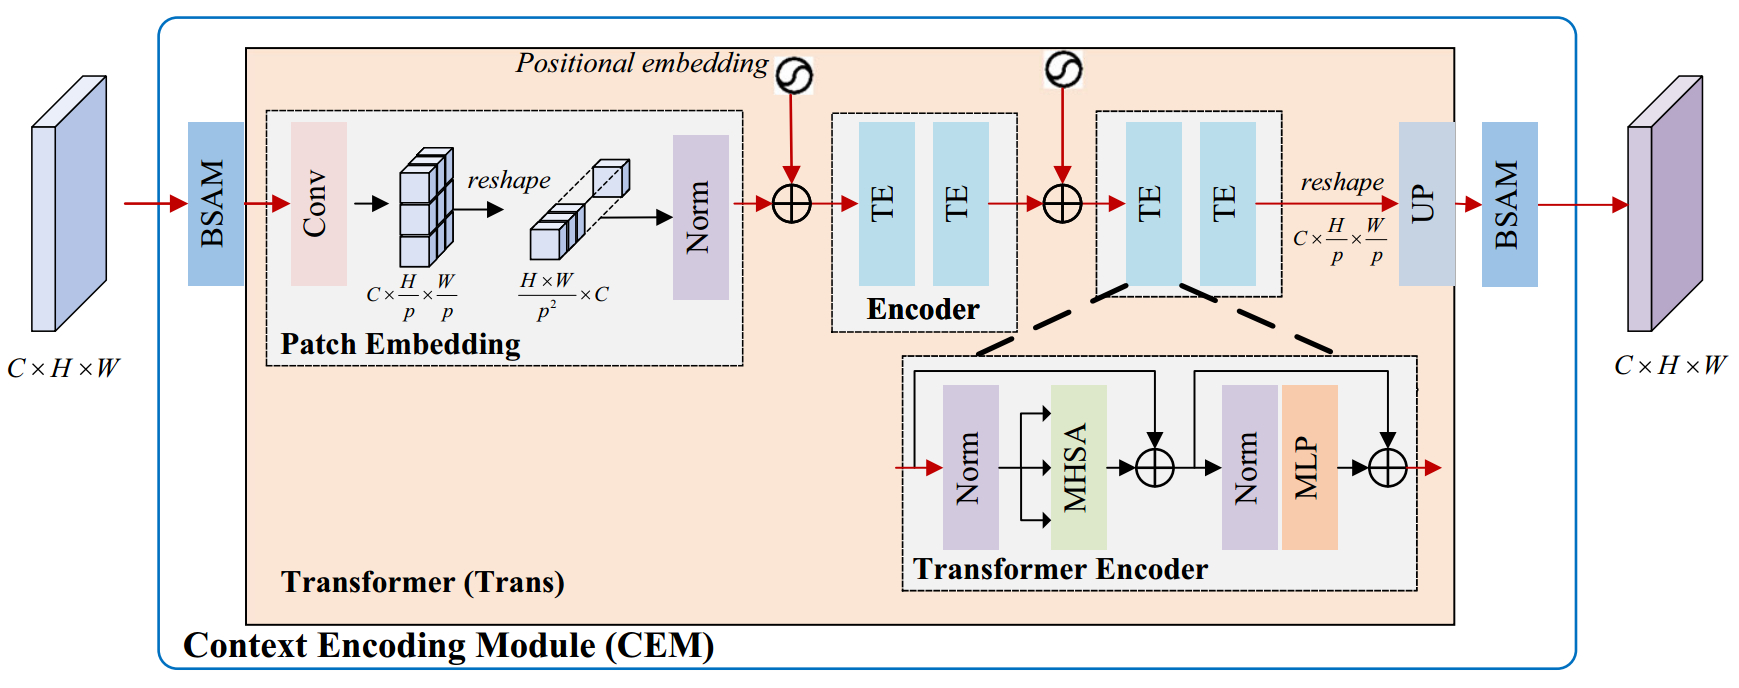
\includegraphics[width=0.7\columnwidth]{picture/LLIE/MCLNet/CEM}
				%\captionsetup{font=scriptsize}
				\caption{
					\label{fig: MCLNet CEM} 
					The architecture of the Context Encoding Module (CEM)
				}
			\end{figure}
			
			MCLNet 由高效特征提取子网络 (EFES) 和上采样子网络 (US) 组成,如 Fig. \ref{fig: MCLNet Overview}所示。具体来说,EFES 由两个部分组成: 规模聚合的瓶块模块 (BSAM) (如 Fig. \ref{fig: MCLNet BSAM})和上下文编码模块 (CEM)(如 Fig. \ref{fig: MCLNet CEM})。它们分别学习多尺度表示和建模全局依赖关系。通过叠加 BSAM,该模型可以从微光图像中获得层次特征。BSAM 的核心部分是一个关注残差多尺度块 (ARMB)。ARMB (见 Fig. \ref{fig: MCLNet ARMB})通过通道注意机制融合不同的尺度特征并对这些特征进行加权。它使我们的模型增强了多尺度学习能力,并突出了有价值的信息。然后,我们应用 CEM 来捕获远程依赖,这是由 Transformer 执行的。此外,为了充分提取网络的纹理和细节信息,我们引入了感知损失函数来引导网络生成高质量的图像。
			
			\subsubsection{Future}
			
			-

		\subsection{(2018.3)CBAM: Convolutional Block Attention Module}
		
		\paragraph{CBAM:卷积块注意模块}
		
		\paragraph{(ECCV 2018)}

		\subsubsection{Research Background}

		-
		
		\subsubsection{Contribution}
		
		作者提出了卷积块的注意力模块 (Convolutional Block Attention Module),简称 CBAM,该模块是一个简单高效的前向卷积神经网络注意力模块。给定一张特征图,CBAM 沿着通道 (channel) 和空间 (spatial) 两个单独的维度依次推断注意力图,然后将注意力图和输入特征图相乘,进行自适应特征细化。因为 CBAM 是一个轻量级的通用模块,可以无缝的集成到任何 CNN 架构中,几乎对效率,算力没有影响,能够实现端到端的训练。
		
		作者的主要贡献有以下三方面:
		
		\begin{itemize}
			\item[(1)] 
			作者提出了一个简单而有效的注意力模块 (CBAM),可以广泛应用于提高 CNN 的表征能力;
			
			\item[(2)]
			作者通过广泛的消融研究验证了注意力模块的有效性;
			
			\item[(3)]
			作者插入了轻量级模块,并验证了各种网络的性能在多个基准测试(ImageNet-1K, MS COCO 和 VOC 2007)上得到了极大的提高。
			
		\end{itemize}	
		
		\subsubsection{Approach}
		
		在该论文中,作者研究了网络架构中的注意力,注意力不仅要告诉我们重点关注哪里,还要提高关注点的表示。 目标是通过使用注意机制来增加表现力,关注重要特征并抑制不必要的特征。为了强调空间和通道这两个维度上的有意义特征,作者依次应用通道和空间注意模块,来分别在通道和空间维度上学习关注什么、在哪里关注。此外,通过了解要强调或抑制的信息也有助于网络内的信息流动。
		主要网络架构也很简单,一个是通道注意力模块,另一个是空间注意力模块,CBAM 就是先后集成了通道注意力模块和空间注意力模块。
		
		Convolutional Block Attention Module (CBAM) 表示卷积模块的注意力机制模块,是一种结合了空间 (spatial) 和通道 (channel) 的注意力机制模块(见Fig. \ref{fig: CBAM-overview})。
		
		\begin{figure}[htbp]
			% read manual to see what [ht] means and for other possible options
			\centering 
			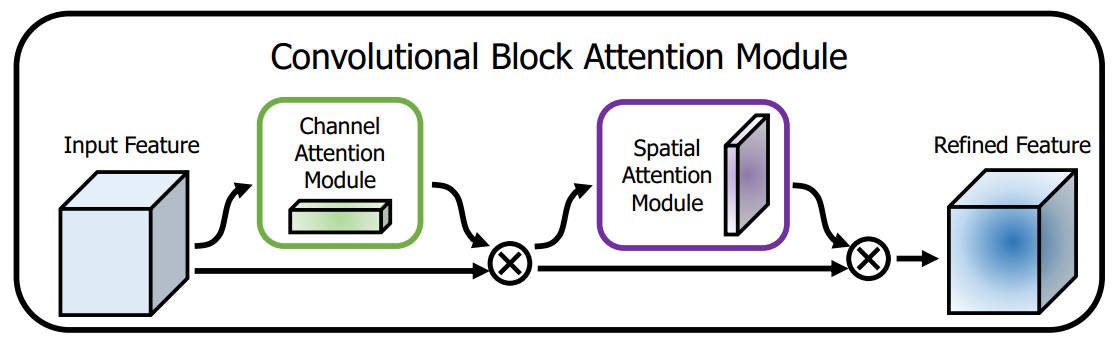
\includegraphics[width=0.7\columnwidth]{picture/LLIE/CBAM/CBAM-overview}
			%\captionsetup{font=scriptsize}
			\caption{
				\label{fig: CBAM-overview} 
				\textbf{The overview of CBAM.} The module has two sequential sub-modules:
				channel and spatial. The intermediate feature map is adaptively refined through
				our module (CBAM) at every convolutional block of deep networks.
			}
		\end{figure}
		
		CBAM 的过程为:给定一个中间特征图,属性为高$H$,宽$W$,维度$C$,作为输入,$\mathbf{F} \in \mathbb{R}^{C \times H \times W}$,CBAM 依次得到一个一维的通道注意力图 $M_c$和一个二维的空间注意力图 $M_s$,整个流程可以概括为: 
		
		\begin{equation}
			\begin{aligned}
				\mathbf{F}^{\prime} = \mathbf{M_c}(\mathbf{F}) \otimes \mathbf{F}, \\
				\mathbf{F}^{\prime\prime} = \mathbf{M_s}(\mathbf{F}^{\prime}) \otimes \mathbf{F}^{\prime}
			\end{aligned}
			\label{eq: CBAM}
		\end{equation}
		
		其中,$\otimes$ 表示对应元素相乘操作。
		
		\paragraph{Channel Attention Module}
		
		\begin{figure}[htbp]
			% read manual to see what [ht] means and for other possible options
			\centering 
			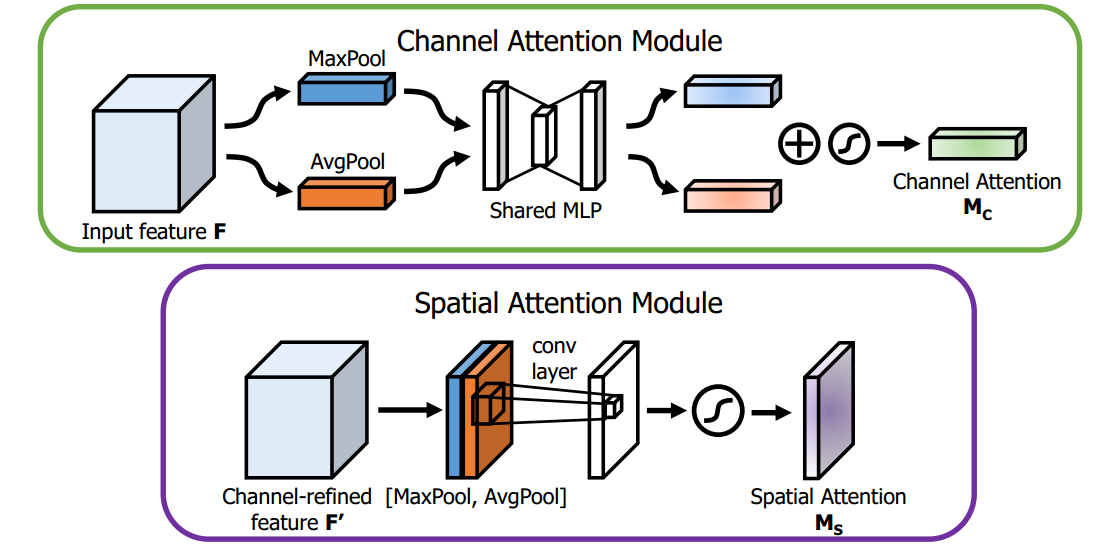
\includegraphics[width=0.7\columnwidth]{picture/LLIE/CBAM/Attention Module}
			%\captionsetup{font=scriptsize}
			\caption{
				\label{fig: Attention Module} 
				\textbf{Diagram of each attention sub-module.} As illustrated, the channel sub-module utilizes both max-pooling outputs and average-pooling outputs with a shared network; the spatial sub-module utilizes similar two outputs that are pooled along the channel axis and forward them to a convolution layer.
			}
		\end{figure}
		
		通道注意力机制 (见Fig. \ref{fig: Attention Module}) 是将特征图在空间维度上进行压缩,得到一个一维矢量后再进行操作。在空间维度上进行压缩时,不仅考虑到了平均值池化 (Average Pooling) 还考虑了最大值池化 (Max Pooling)。平均池化和最大池化可用来聚合特征映射的空间信息,送到一个共享网络,压缩输入特征图的空间维数,逐元素求和合并,以产生通道注意力图。单就一张图来说,通道注意力,关注的是这张图上哪些内容是有重要作用的。平均值池化对特征图上的每一个像素点都有反馈,而最大值池化在进行梯度反向传播计算时,只有特征图中响应最大的地方有梯度的反馈。通道注意力机制可以表达为:
		
		\begin{equation}
			\begin{aligned}
				\mathbf{M_c}(\mathbf{F}) &= \sigma \left( MLP(AvgPool(\mathbf{F})) + MLP(MaxPool(\mathbf{F})) \right) \\
				&= \sigma \left( \mathbf{W_1}(\mathbf{W_0}(\mathbf{F_{avg}^c})) + \mathbf{W_1}(\mathbf{W_0}(\mathbf{F_{max}^c})) \right)	
			\end{aligned}
			\label{eq: Channel Attention Module}
		\end{equation}
		
		其中,$\sigma$为 sigmoid 操作。
		
		\paragraph{Spatial Attention Module}
		
		空间注意力机制 (见Fig. \ref{fig: Attention Module}) 是对通道进行压缩,在通道维度分别进行了平均值池化和最大值池化。MaxPool的操作就是在通道上提取最大值,提取的次数是高乘以宽;AvgPool的操作就是在通道上提取平均值,提取的次数也是是高乘以宽;接着将前面所提取到的特征图(通道数都为1)合并得到一个2通道的特征图。
		
		\begin{equation}
			\begin{aligned}
				\mathbf{M_s}(\mathbf{F}) &= \sigma \left( f^{7 \times 7}([AvgPool(\mathbf{F});MaxPool(\mathbf{F})]) \right) \\
				&= \sigma \left( f^{7 \times 7}([\mathbf{F^s_{avg}};\mathbf{F^s_{max}}]) \right)
			\end{aligned}
			\label{eq: Spatial Attention Module}
		\end{equation}
		
		其中,$7 \times 7$表示卷积核的大小。
		
		\subsubsection{Future}
		
		-
		
		\subsection{(2023)SCConv: Spatial and Channel Reconstruction Convolution for Feature Redundancy}
		
		\paragraph{SCConv:特征冗余的空间和信道重建卷积 }
		
		\paragraph{(CVPR 2023)}
		
		\subsubsection{Research Background}
		
		-
		
		\subsubsection{Contribution}
		
		本文作者提出了一种名为 SCConv(Spatial and Channel reconstruction Convolution, 空间和通道重建卷积) 的卷积模块,目的是减少卷积神经网络中特征之间的空间和通道冗余,从而压缩CNN模型并提高其性能。
		
		作者设计的 SCConv 模块,包含两个单元。一个名为 SRU (Spatial Reconstruction Unit, 空间重构单元) ,一个名为 CRU (Channel Reconstruction Unit, 通道重构单元) 。其中 SRU 通过 分离-重构方法 来减少空间冗余,CRU 则使用 分割-转换-融合方法 来减少通道冗余。这两个单元协同工作,以减少CNN中特征的冗余信息。
		
		作者指出,SCConv 是一种可以直接替代标准卷积操作的插件式卷积模块,可以应用于各种卷积神经网络中,从而降低冗余特征并减少计算复杂性。
		
		在后续的实验中,作者认为相对于其他流行的 SOTA 方法,他们提出的 SCConv 可以以更低的计算成本获得更高的准确率。
		
		\subsubsection{Approach}
		
		如 Fig. \ref{fig: SCConv} 所示,SCConv 由两个单元组成,即空间重构单元 (SRU) 和信道重构单元 (CRU) ,两个单元按顺序排列。输入的特征 $X$ 先经过 SRU,得到空间细化的特征 $X^{w}$。再经过 CRU,得到通道提炼的特征 $Y$ 作为输出。
		
		\begin{figure}[htbp]
			% read manual to see what [ht] means and for other possible options
			\centering 
			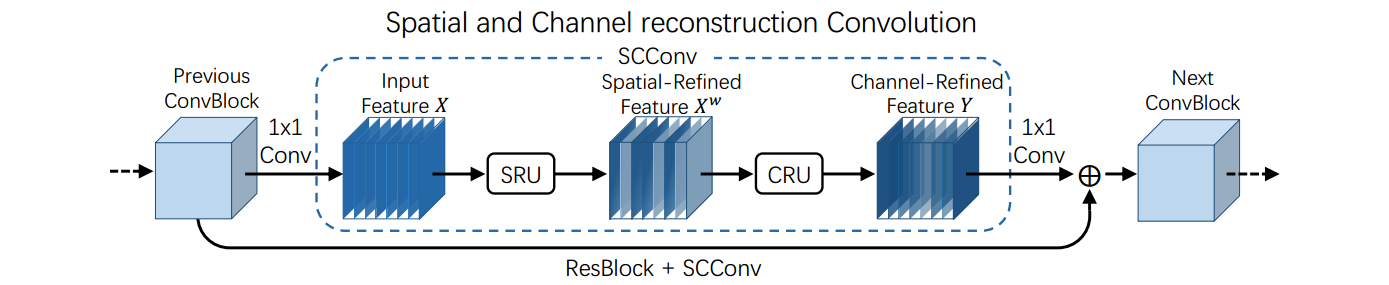
\includegraphics[width=\columnwidth]{picture/LLIE/SCConv/SCConv}
			%\captionsetup{font=scriptsize}
			\caption{
				\label{fig: SCConv} 
				The architecture of SCConv integrated with Spatial Reconstruction Unit (SRU) and Channel Reconstruction Unit (CRU). This figure shows the exact position of our SCConv module within a ResBlock.
			}
		\end{figure}
		
		SCConv 模块利用了特征之间的空间冗余和信道冗余,模块可以无缝集成到任何 CNN 框架中,减少特征之间的冗余,提高 CNN 特征的代表性。
		
		作者通过实验发现先使用 SRU 再使用 CRU 的效果最好。
		
		\paragraph{SRU}
		
		在作者的设计中,该单元采用\textbf{分离-重构}的方法。
		
		\textbf{分离}操作的目的是将信息量大的特征图从信息量小的特征图中分离出来,与空间内容相对应。作者使用组归一化 (Group Normalization) 里的缩放因子来评估不同特征图中的信息含量。
		
		\begin{figure}[htbp]
			% read manual to see what [ht] means and for other possible options
			\centering 
			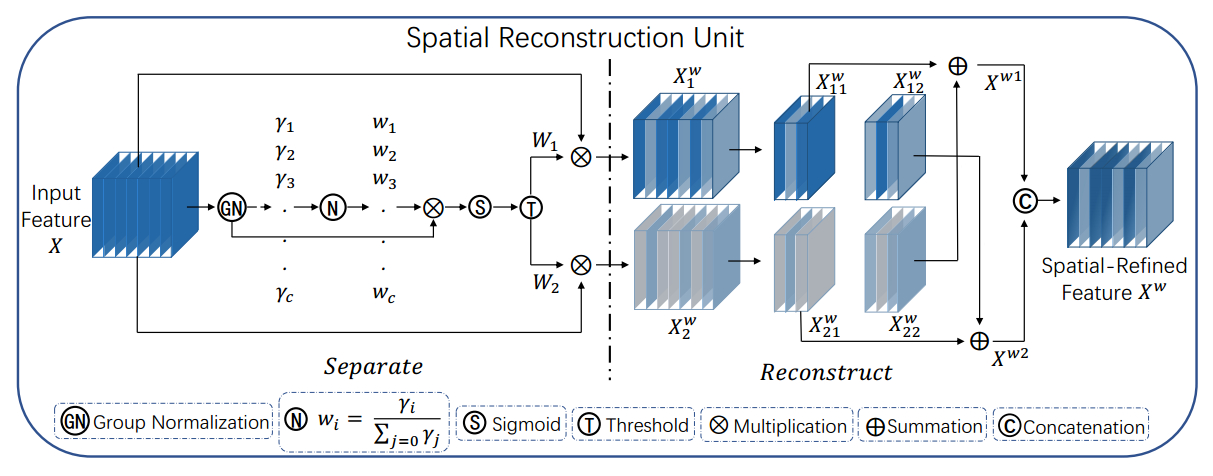
\includegraphics[width=\columnwidth]{picture/LLIE/SCConv/Spatial Reconstruction Unit}
			%\captionsetup{font=scriptsize}
			\caption{
				\label{fig: Spatial Reconstruction Unit} 
				The architecture of Spatial Reconstruction Unit.
			}
		\end{figure}
		
		\begin{equation}
			\begin{aligned}
				X_{out} = \textbf{GN}(X) = \gamma \frac{X-\mu}{\sqrt{\sigma^2 + \varepsilon}} + \beta \\
				W_{\gamma} = {w_i} = \frac{\gamma_i}{\sum_{j=1}^{C} \gamma_j}, \ i,\ j = 1, 2, \cdots, C \\
				W = \textbf{Gate}(\textbf{Sigmoid}(W_{\gamma}(\textbf{GN}(X))))				
			\end{aligned}
			\label{eq: SRU}
		\end{equation}
		
		其中,$\mu$, $\sigma$是均值和标准差,$\gamma$, $\beta$ 是可训练的变量,$\varepsilon$ 是用于保证稳定性的极小常数。更大的 $\gamma$ 代表像素之间更大的变化,也就是更丰富的空间信息。
		
		\textbf{重构}操作是将信息量较多的特征和信息量较少的特征相加,生成信息量更多的特征并节省空间。具体的操作是交叉重建,将加权后的两个不同信息特征合并,得到 $X^{w1}$ 和 $X^{w2}$,连接起来后得到空间细化特征图 $X^{w}$。
		
		\begin{equation}
			\left\{
			\begin{aligned}
				&X_{1}^{w} = W_1 \otimes X , \\
				&X_{2}^{w} = W_2 \otimes X , \\
				&X_{11}^{w} \oplus X_{22}^{w} = X^{w1} , \\
				&X_{21}^{w} \oplus X_{12}^{w} = X^{w2} , \\
				&X^{w1} \cup X^{w2} = X^{w}.
			\end{aligned}
			\right.
		\end{equation}
		
		其中 $\otimes$ 是元素乘法,$\oplus$是元素加法,$\cup$ 是求并集。
		经过 SRU 处理后,信息量大的特征从信息量小的特征中分离出来,减少了空间维度上的冗余特征。
		\paragraph{CRU}
		
		在作者的设计中,该单元采用\textbf{分割-转换-融合}的方法。
		
		\begin{figure}[htbp]
			% read manual to see what [ht] means and for other possible options
			\centering 
			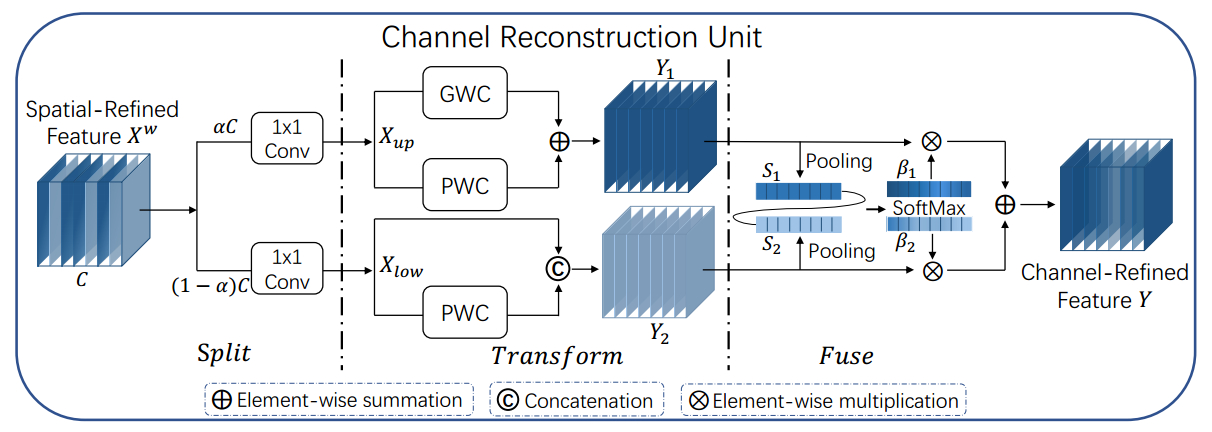
\includegraphics[width=\columnwidth]{picture/LLIE/SCConv/Chanel Reconstruction Unit}
			%\captionsetup{font=scriptsize}
			\caption{
				\label{fig: Chanel Reconstruction Unit} 
				The architecture of Chanel Reconstruction Unit.
			}
		\end{figure}
		
		\textbf{分割}操作将输入的空间细化特征 $X^{w}$ 分割为两部分:一部分的通道数是 $\alpha C$,另一部分的通道数是 $(1-\alpha) C$,其中 $\alpha$ 是超参数且 $0 \textless \alpha \textless 1$。随后对两组特征的通道数使用 $1 \times 1$ 卷积核进行压缩,分别得到 $X_{up}$ 和 $X_{low}$。
		
		\textbf{转换}
		
		\textbf{融合}
		
		\subsubsection{Future}
		
		-
		
		\renewcommand{\refname}{References}
		
		
		%	\begin{thebibliography}{00}
			
			%		\bibitem{b1}\label{cite:b1}
			%		W. Wang, C. Wei, W. Yang and J. Liu, "GLADNet: Low-Light Enhancement Network with Global Awareness," 2018 13th IEEE International Conference on Automatic Face \& Gesture Recognition (FG 2018), Xi'an, China, 2018, pp. 751-755, DOI: 10.1109/FG.2018.00118.
			
			%		\bibitem{b2}\label{cite:b2}
			%		A.\ Mahajan, K.\ Somaraj and M. Sameer, "Adopting Artificial Intelligence Powered ConvNet To Detect Epileptic Seizures," 2020 IEEE-EMBS Conference on Biomedical Engineering and Sciences (IECBES), Langkawi Island, Malaysia, 2021, pp. 427-432, DOI: 10.1109/IECBES48179.2021.9398832.
			
			%		\bibitem{Cyr}
			%		N.\ Cyr, M.\ T$\hat{e}$tu, and M.\ Breton,
			% "All-optical microwave frequency standard: a proposal,"
			%		IEEE Trans.\ Instrum.\ Meas.\ \textbf{42}, 640 (1993).
			
			
			
			%	\end{thebibliography}
		
		\bibliographystyle{unsrt}
		\bibliography{reference}
		
		
	\end{document}
